\RCS$Revision: 326816 $
\RCS$HeadURL: svn+ssh://svn.cern.ch/reps/tdr2/papers/SUS-15-005/trunk/SUS-15-005.tex $
\RCS$Id: SUS-15-005.tex 326816 2016-02-19 20:36:18Z sakuma $

\newlength\cmsFigWidth
\ifthenelse{\boolean{cms@external}}{\setlength\cmsFigWidth{0.85\columnwidth}}{\setlength\cmsFigWidth{0.4\textwidth}}
\ifthenelse{\boolean{cms@external}}{\providecommand{\cmsLeft}{top\xspace}}{\providecommand{\cmsLeft}{left\xspace}}
\ifthenelse{\boolean{cms@external}}{\providecommand{\cmsRight}{bottom\xspace}}{\providecommand{\cmsRight}{right\xspace}}

\newcommand{\kfactor}{\ensuremath{k\text{-factor}}\xspace}
\newcommand{\kfactors}{\ensuremath{k\text{-factors}}\xspace}
\newcommand{\njet}{\ensuremath{n_{\text{jet}}}\xspace}
\newcommand{\njetlow}{\ensuremath{2 \leq \njet \leq 3}\xspace}
\newcommand{\njethigh}{\ensuremath{\njet \geq 4}\xspace}
\newcommand{\nb}{\ensuremath{n_{\text{b}}}\xspace}
\newcommand{\alphat}{\ensuremath{\alpha_{\text{T}}}\xspace}
\newcommand{\alphatcut}{\ensuremath{\alpha_{\text{T}}^{\text{cut}}}\xspace}
\newcommand{\htalphat}{\texttt{HT\_AlphaT}\xspace}
\newcommand{\photon}{\texttt{Photon}\xspace}
\newcommand{\muht}{\texttt{Mu\_HT}\xspace}
\newcommand{\httrigger}{\texttt{HT}\xspace}
\newcommand{\mt}{\ensuremath{M_{\textrm T}}\xspace}
\newcommand{\gj}{\ensuremath{\gamma} + jets\xspace}
\newcommand{\mj}{\ensuremath{\mu} + jets\xspace}
\newcommand{\mmj}{\ensuremath{\mu\mu} + jets\xspace}
\newcommand{\npre}{\ensuremath{N_{\textrm{pred}}}\xspace}
\newcommand{\nobs}{\ensuremath{N_{\textrm{obs}}}\xspace}
\newcommand{\njets}{\ensuremath{N_{\textrm{jet}}}\xspace}
\newcommand{\sq}{\ensuremath{\tilde{\rm q}}\xspace}
\newcommand{\st}{\ensuremath{\tilde{\rm t}}\xspace}
\newcommand{\gl}{\ensuremath{\tilde{\rm g}}\xspace}
\newcommand{\dht}{\ensuremath{\Delta\scalht}\xspace}
\newcommand{\ewk}{\ensuremath{\mathrm{EWK}}\xspace}
\newcommand{\qcd}{\ensuremath{\mathrm{QCD}}\xspace}
\newcommand{\fZinv}[1]{\ensuremath{f_{\rm Zinv}^{#1}}\xspace}
\newcommand{\zInv}[1]{\ensuremath{Z_{\rm inv}^{#1}}\xspace}
\newcommand{\meanHt}[1]{\ensuremath{\langle \HT \rangle^{#1}}\xspace}
\newcommand{\lk}[2]{\ensuremath{L^{\rm #1}_{\rm #2}}\xspace}
\newcommand{\sep}{\ensuremath{68^{\mathrm{th}}}\xspace}
\newcommand{\partonht}{\ensuremath{\scalht^{\rm parton}}\xspace}
\newcommand{\meff}{\ensuremath{M_{\rm eff}}\xspace}
\newcommand{\mhttt}{\ensuremath{\hslash_{\rm T}^{TT}}\xspace}


\newcommand\rs{\raisebox{1.0ex}[-1.0ex]}
\newcommand{\ra}{\ensuremath{\rightarrow}}
\newcommand{\znunu}{\ensuremath{{\text Z} \ra \nu\bar{\nu}}\xspace}
\newcommand{\zll}{\ensuremath{{\text Z} \ra \ell\ell}\xspace}
\newcommand{\zmumu}{\ensuremath{{\text Z} \ra \mu\mu}\xspace}
\newcommand{\zee}{\ensuremath{{\text Z} \ra ee}\xspace}
\newcommand{\wmunu}{\ensuremath{{\text W} \ra \mu\nu}}
\newcommand{\wtaunu}{\ensuremath{{\text W} \ra \tau\nu}}
\newcommand{\dphi}{\ensuremath{\Delta \phi}}
\newcommand{\dphijj}{\ensuremath{\Delta \phi_{ j1,j2}}}
\newcommand{\Pt}{\ensuremath{{p_{\text T}}}\xspace}
\newcommand{\pts}{\ensuremath{p_{\text T}{\text s}}\xspace}
\newcommand{\Et}{\ensuremath{{E_{\text T}}}\xspace}
\newcommand{\ptjf}{\ensuremath{p_{\rm T}^{ {\rm j}_1} }}
\newcommand{\ptjs}{\ensuremath{p_{\rm T}^{ {\rm j}_2} }}
\newcommand{\ptjt}{\ensuremath{p_{\rm T}^{ {\rm j}_3} }}
\newcommand{\etajf}{\ensuremath{\eta^{ {\rm j}_1} }}
\newcommand{\etajs}{\ensuremath{\eta^{ {\rm j}_2} }}
\newcommand{\etajt}{\ensuremath{\eta^{ {\rm j}_3} }}
\newcommand{\ttj}{\ensuremath{\rm{t}\bar{\rm{t}} + jets}\xspace}
\newcommand{\wj}{\ensuremath{\rm W + \textrm{jets}}\xspace}
\newcommand{\wej}{\ensuremath{{\rm W}(\rightarrow{\rm e}\nu) + \textrm{jets}}\xspace}
\newcommand{\wmj}{\ensuremath{{\rm W}(\rightarrow\mu\nu) + \textrm{jets}}\xspace}
\newcommand{\zj}{\ensuremath{{\rm Z} + \textrm{jets}}\xspace}
\newcommand{\zmmj}{\ensuremath{{\rm Z}(\rightarrow\mu\mu) + \textrm{jets}}\xspace}
\newcommand{\zeej}{\ensuremath{{\rm Z}(\rightarrow{\rm ee}) + \textrm{jets}}\xspace}

\newcommand{\al}{\ensuremath{\alpha}}
\newcommand{\alt}{\ensuremath{\alpha_{\text{T}}}\xspace}
\newcommand{\etaabs}{\ensuremath{|\eta|}}
%\newcommand{\gev}{\ensuremath{\mathrm{\,Ge\kern -0.1em V}}}
\newcommand{\pb}{\ensuremath{pb^{-1}}}
\newcommand{\mjj}{\ensuremath{M_{\text{inv}}^{j1,j2}}}
%\newcommand{\ttbar}{\ensuremath{t\bar{t}}}
\newcommand{\chiznew}{\ensuremath{\chi^{0}}\xspace}
\newcommand{\chipnew}{\ensuremath{\chi^{+}}\xspace}
\newcommand{\sQuanew}{\ensuremath{\tilde{\rm q}}\xspace}
\newcommand{\sGlunew}{\ensuremath{\tilde{\rm g}}\xspace}
\newcommand{\ttNew}{\ensuremath{\rm{t}\bar{\rm{t}}}\xspace}
\newcommand{\tev}{\TeV}
%<TW date="30/10/2010">
%\newcommand{\Et}{E_{T}}
\newcommand{\combIso}{Iso_{\textrm{comb.}}}
\renewcommand{\arraystretch}{1.2}
\newcommand{\bigNum}[2]{#1 \, \times \, 10 \, ^{#2}}
%</TW>

\newcommand{\raT}{\ensuremath{R_{\alt}}}
\newcommand{\RaT}{\ensuremath{R_{\alt}}\xspace}

\newcommand{\Ttwocc}{\ensuremath{\text{pp}\,\ra\,\sTop\sTop^{*}\,\ra\,\text{c}\chiz\,\bar{\text{c}}\chiz}}
\newcommand{\Ttwodegen}{\ensuremath{\text{pp}\,\ra\,\sTop\sTop^{*}\,\ra\,\text{b}ff'\chiz \,\text{b}ff'\chiz}}
\newcommand{\Ttwobw}{\ensuremath{\text{pp}\,\ra\,\sTop\sTop^{*}\,\ra\,\text{b}W\chiz \,\bar{\text{b}}W\chiz}}
\newcommand{\Ttwott}{\ensuremath{\text{pp}\,\ra\,\sTop\sTop^{*}\,\ra\,\text{t}\chiz\,\bar{\text{t}}\chiz}}
\newcommand{\Ttwobb}{\ensuremath{\text{pp}\,\ra\,\sBot\sBot^{*}\,\ra\,\text{b}\chiz\,\bar{\text{b}}\chiz}}
\newcommand{\Ttwoqq}{\ensuremath{\text{pp}\,\ra\,\sQua\sQua^{*}\,\ra\,\text{q}\chiz\,\bar{\text{q}}\chiz}}
\newcommand{\Tonebbbb}{\ensuremath{\text{pp}\,\ra\,\sGlunew\sGlunew^{*}\,\ra\,\bar{\text{b}}\text{b}\chiz\,\bar{\text{b}}\text{b}\chiz}}
\newcommand{\Toneqqqq}{\ensuremath{\text{pp}\,\ra\,\sGlunew\sGlunew^{*}\,\ra\,\bar{\text{q}}\text{q}\chiz\,\bar{\text{q}}\text{q}\chiz}}
\newcommand{\Tonetttt}{\ensuremath{\text{pp}\,\ra\,\sGlunew\sGlunew^{*}\,\ra\,\bar{\text{t}}\text{t}\chiz\,\bar{\text{t}}\text{t}\chiz}}

\newcommand\T{\rule{0pt}{2.6ex}}
\newcommand\B{\rule[-1.2ex]{0pt}{0pt}}

\def\eslash{{\hbox{$E$\kern-0.6em\lower-.05ex\hbox{/}\kern0.10em}}}
\def\vecmet{\mbox{$\vec{\eslash}_T$}} %missing ET vector
\def\vecet{\mbox{$\vec{E}_\text{T}$}} % ET vector
\def\MET{\mbox{$\eslash_\text{T}$}\xspace}
%\def\met{\mbox{$\eslash_\text{T}$}\xspace}
\def\met{\mbox{$E_\text{T}^{\rm miss}$}\xspace}
\def\pfmet{\mbox{$\eslash_\text{T}^{\rm PF}$}\xspace}
\def\mex{\mbox{$\eslash_\text{x}$}} %missing Ex
\def\mey{\mbox{$\eslash_\text{y}$}} %missing Ey
\def\mepar{\mbox{$\eslash_\parallel$}}
\def\meperp{\mbox{$\eslash_\perp$}}
\def\Zmm{Z \rightarrow \mu\mu}
\def\metvec{\mbox{$\vec{\met}$}\xspace}
\def\metvecrec{\mbox{$\vec{\met}^{\rm rec}$}\xspace}
\def\metvecgen{\mbox{$\vec{\met}^{\rm gen}$}\xspace}
\def\metgen{\mbox{$\met^{\rm gen}$}\xspace}
\def\metparl{\mbox{$\mepar^{\rm rec}$}\xspace}
\def\metperp{\mbox{$\meperp^{\rm rec}$}\xspace}
\def\deltamet{\mbox{$\Delta\met$}\xspace}
\def\pthat{\mbox{$\hat{p}_T$}\xspace}
\def\hslash{{\hbox{$H$\kern-0.8em\lower-.05ex\hbox{/}\kern0.10em}}}
\def\MHT{\mbox{$\hslash_\text{T}$}\xspace}
%\def\mht{\mbox{$\hslash_\text{T}$}\xspace}
\def\mht{\mbox{$H_{\rm T}^{\rm miss}$}\xspace}
\def\mhtvec{\mbox{$\vec{H}_{\rm T}^{\rm miss}$}\xspace}
%\def\mhtmet{\mbox{$\hslash_\text{T} / \eslash_\text{T}$}\xspace}
\def\mhtmet{\mbox{$\mht / \met$}\xspace}
\def\mhtmetmiss{\mbox{$\H_\text{T}^{\rm miss} / \E_\text{T}^{\rm miss}$}\xspace}
%\def\rmhtmet{\mbox{$R_{\hslash_\text{T} / \eslash_\text{T}}$}\xspace}
\def\rmhtmet{\mbox{$R_{\mht / \met}$}\xspace}
\def\sumet{\mbox{$\sum \rm{E}_\text{T}$}\xspace}
\def\scalht{\mbox{$H_\text{T}$}\xspace}
\def\etmiss{\mbox{$\eslash_\text{T}$}\xspace}
\def\htmiss{\mbox{$\hslash_\text{T}$}\xspace}
\def\mtt{\mbox{$\rm{M}_\text{T2}$}\xspace}
\def\rmec{\mbox{$R_{\mht/\met}$}\xspace}
\def\bdphi{\mbox{$\Delta\phi^{*}_{\rm min}$}\xspace}
\def\dphimhtj{\mbox{$\Delta\phi(j_{1234}, \mht)_{\rm min}$}\xspace}
\def\bigeslash{{\hbox{$E$\kern-0.38em\lower-.05ex\hbox{/}\kern0.10em}}}
\def\bigmet{\mbox{$\bigeslash_T$}}
\def\bighslash{{\hbox{$H$\kern-0.6em\lower-.05ex\hbox{/}\kern0.10em}}}
\def\bigmht{\mbox{$\bighslash_T$}}
\def\incl{\includegraphics[width=0.49\linewidth]}
\def\inclrot{\includegraphics[angle=90,width=0.47\linewidth]}
\def\INCL{\includegraphics[angle=90,width=0.45\linewidth]}
\def\Incl{\includegraphics[angle=90,width=0.60\linewidth]}
\def\cls{\mbox{CL$_s$}\xspace}
\def\nj{\ensuremath{n_{\mathrm{jet}}}}
\def\nb{\ensuremath{n_{\mathrm{b}}}}

\newcommand{\zero}{\ensuremath{\phantom{0}}}


\cmsNoteHeader{SUS-15-005\_twiki}

\title{Additional (conference/seminar) material for SUS-15-005 }

\date{\today}

\abstract{This document contains the public material aimed at
  conference and seminar speakers for the search ``A search for new
  phenomena in pp collisions at $\sqrt{s} = 13\TeV$ in final states
  with missing transverse momentum and at least one jet using the
  \alphat variable'' (SUS-15-005).}

\hypersetup{ 
  pdfauthor={Mark Baber, Robert Bainbridge, Freya Blekman, Oliver
    Buchmueller, Stefano Casasso, Matthew Citron, Adam Elwood, Henning
    Flaecher, Aran Garcia-Bellido, Christian Laner, Kin Ho Lo, Sarah
    Alam Malik, Bjoern Penning, Tai Sakuma, Dominic Smith, Alex
    Tapper},
  pdftitle={A search for new phenomena in pp collisions at 13 TeV in
  final states with missing transverse momentum and at least one jet
  using the AlphaT variable},
  pdfsubject={CMS},
  pdfkeywords={CMS, jets, missing transverse momentum, supersymmetry,
    dark matter, AlphaT}, 
}

\maketitle


\clearpage
\begin{figure}[tbhp]
    \caption{ 
    The performance of the $\Delta\phi*_{\mathrm{min}}$ variable in black compared to the ``canonical'' $\Delta\phi$ 
    considering all jets in the event ($\Delta\phi(j_{\mathrm{all}},H_{\mathrm{T}}^{miss})$) in red, 
    expressed in terms of efficiency for events from QCD and background with genuine missing transverse momentum (T1tttt model) 
    for several cut values, on the left (right) plot. 
    The black and red stars identify respectively the $\Delta\phi*_{\mathrm{min}}>0.5$ and $\Delta\phi(j_{\mathrm{all}},H_{\mathrm{T}}^{miss})>0.5$ working points. 
    \label{fig:bDPhi-ROC} }
  \begin{center}
     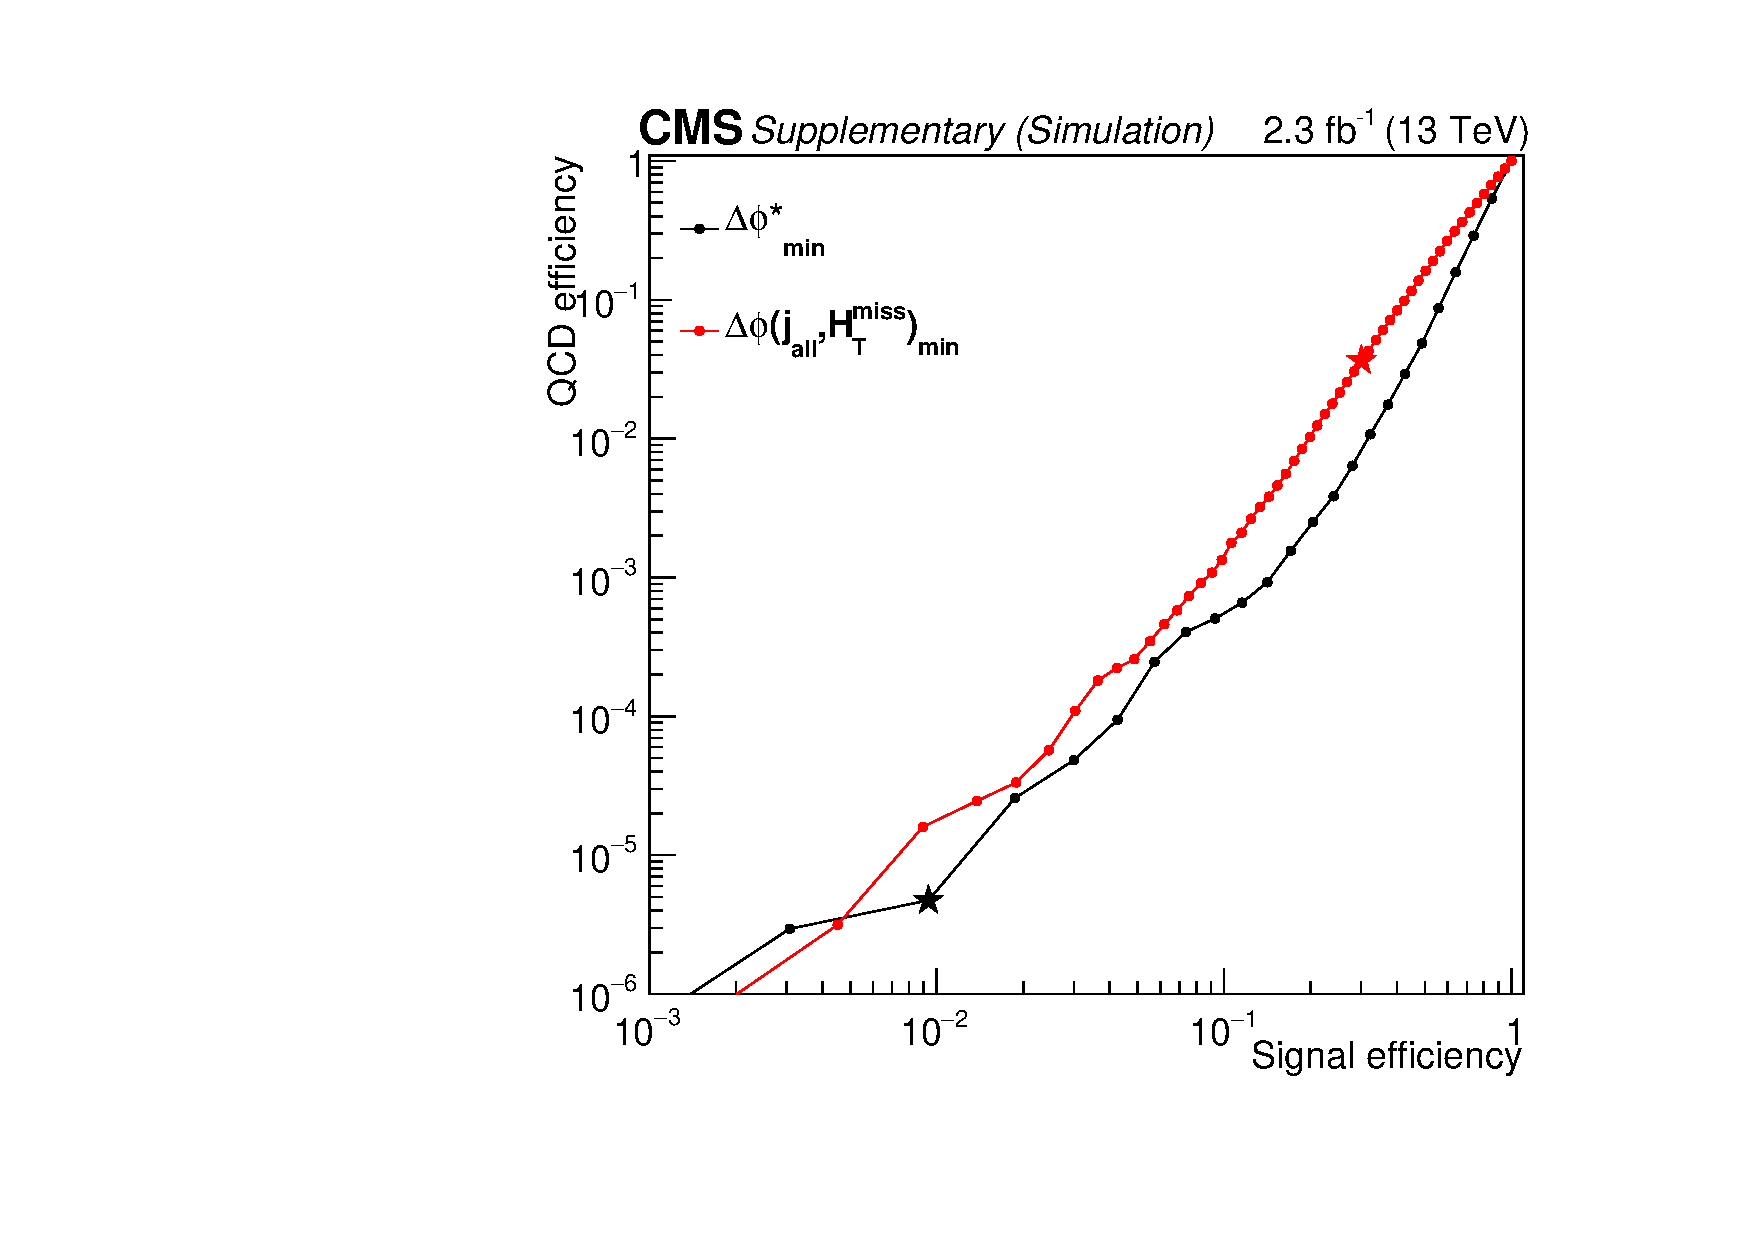
\includegraphics[width=0.48\textwidth]{Supplementary/ewk_ht800_aux} ~~
     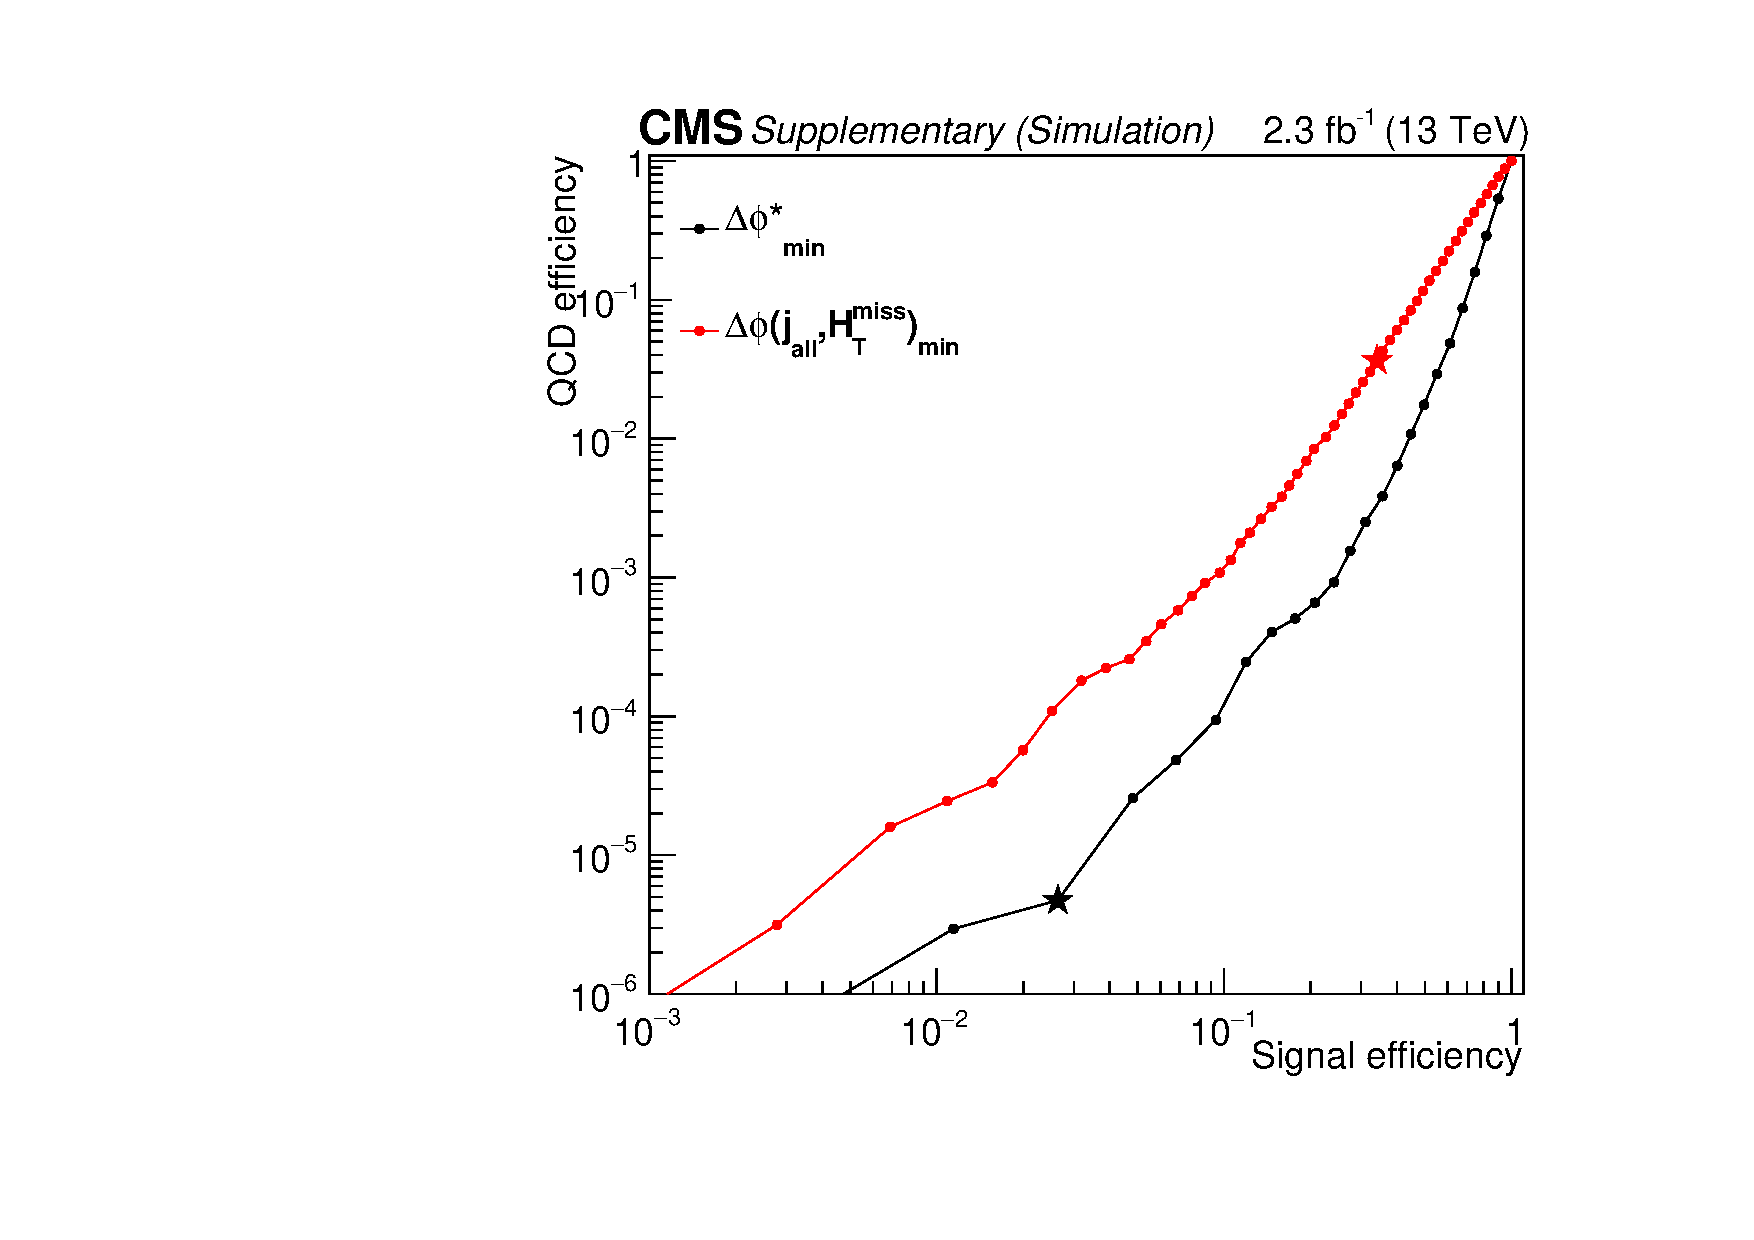
\includegraphics[width=0.48\textwidth]{Supplementary/T1tttt_uncomp_ht800_aux}
  \end{center}
\end{figure}



\clearpage
\begin{figure}[tbhp]
    \caption{ 
    The contribution of the multijet background relative to the sum of
    the non-multijet backgrounds as a function of the $H_{\mathrm{T}}$
    bin (x-axis) and $n_{\mathrm{jet}}$ bin (y-axis), based on
    estimates obtained from data control regions. 
    The empty bins are not used in the analysis because they are
    kinematically not accessible.  
    \label{fig:qcd-rel-cont} }
  \begin{center}
     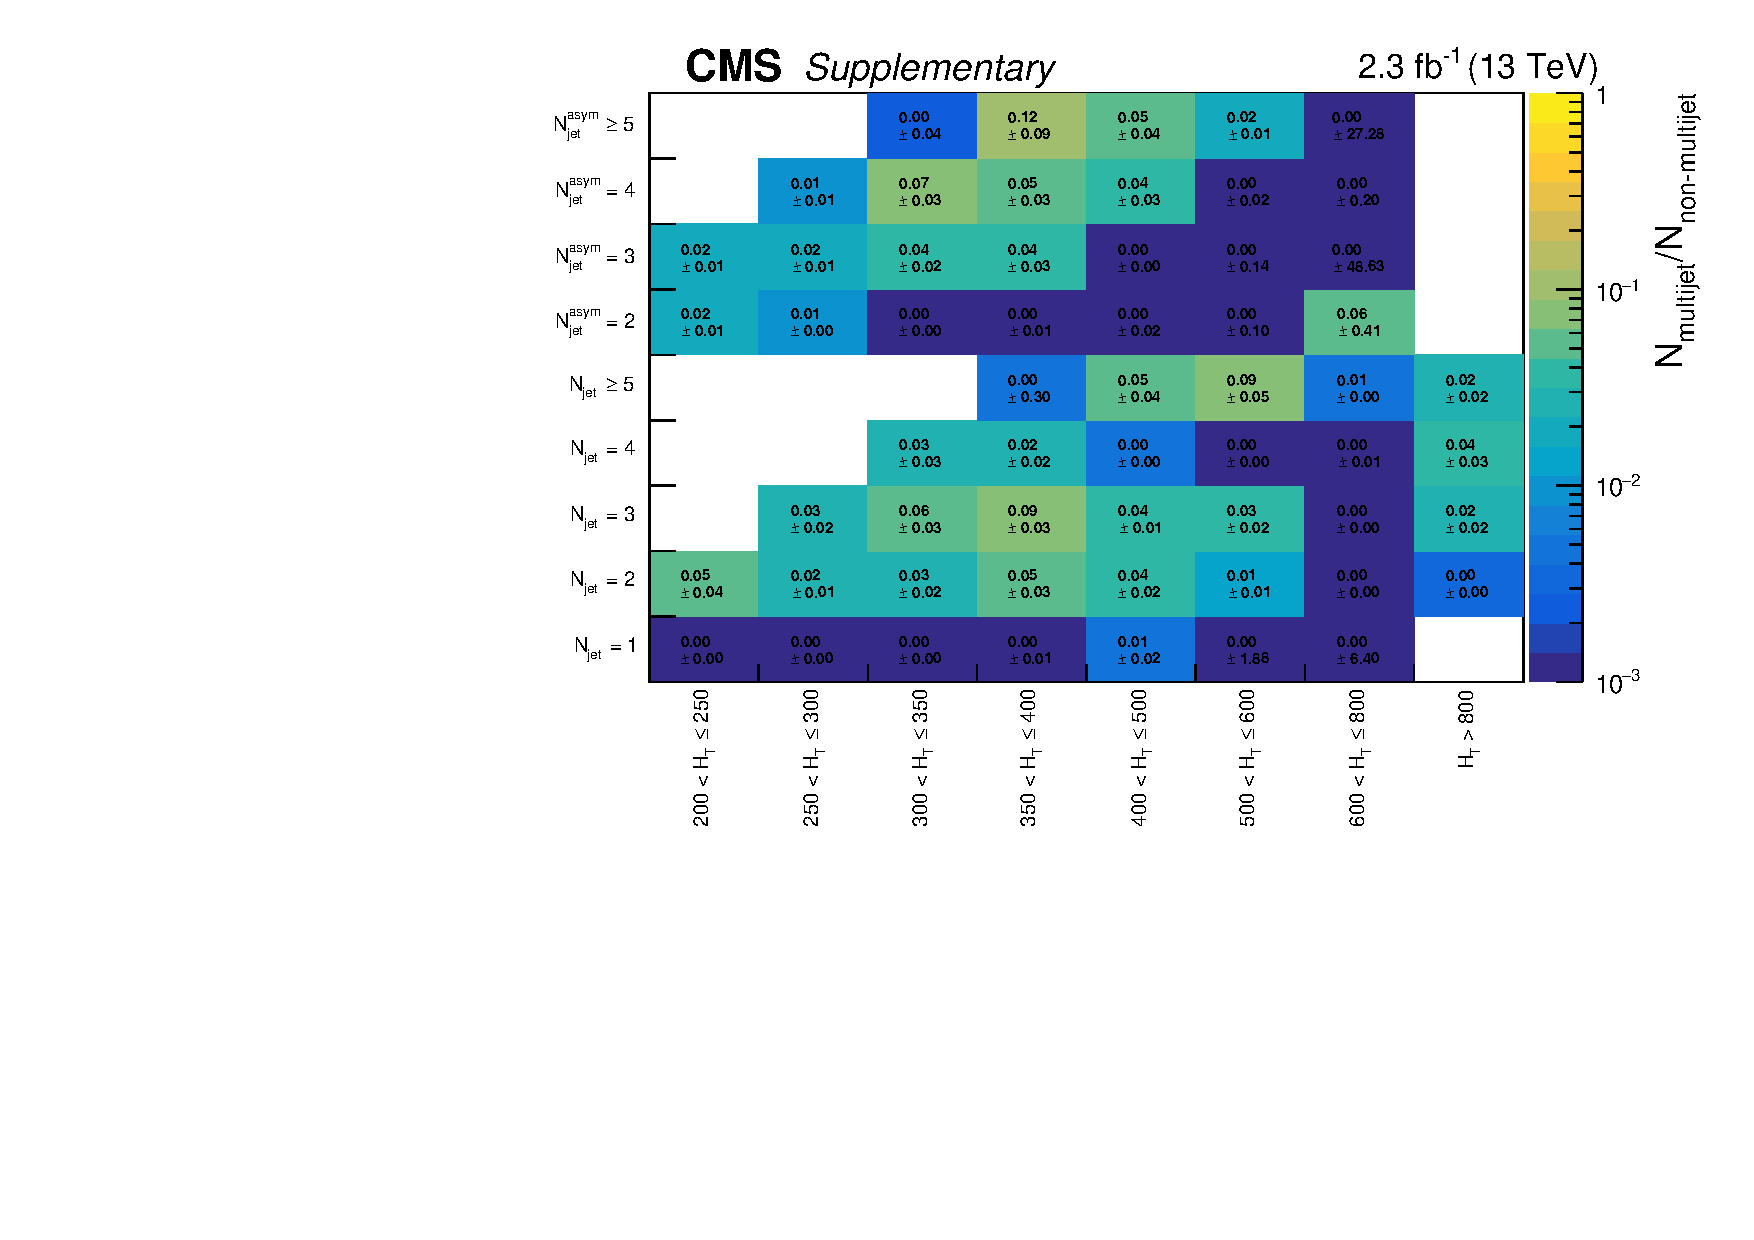
\includegraphics[width=0.5\textwidth]{Supplementary/QCDRelCont_aux}
  \end{center}
\end{figure}



\clearpage
\begin{figure}[tbhp]
    \caption{ 
  Data-derived test of the $\alpha_{\mathrm{T}}$ extrapolation for the symmetric (left) and asymmetric (right) jet categories. 
  In this test, the data yield in the \mj sample with $\alpha_{\mathrm{T}}>0.5$ ($N_{\mathrm{obs}}$) 
  is compared with the prediction obtained from the \mj sample with $\alpha_{\mathrm{T}}<0.5$ multiplied by the corresponding 
  transfer factor computed in simulation ($N_{\mathrm{pred}}$). 
  A systematic uncertainty (grey band) is derived, as a function of $H_{\mathrm{T}}$ and separately for symmetric and asymmetric categories, 
  to cover the non-closure. 
    \label{fig:CT-alphaT} }
  \begin{center}
     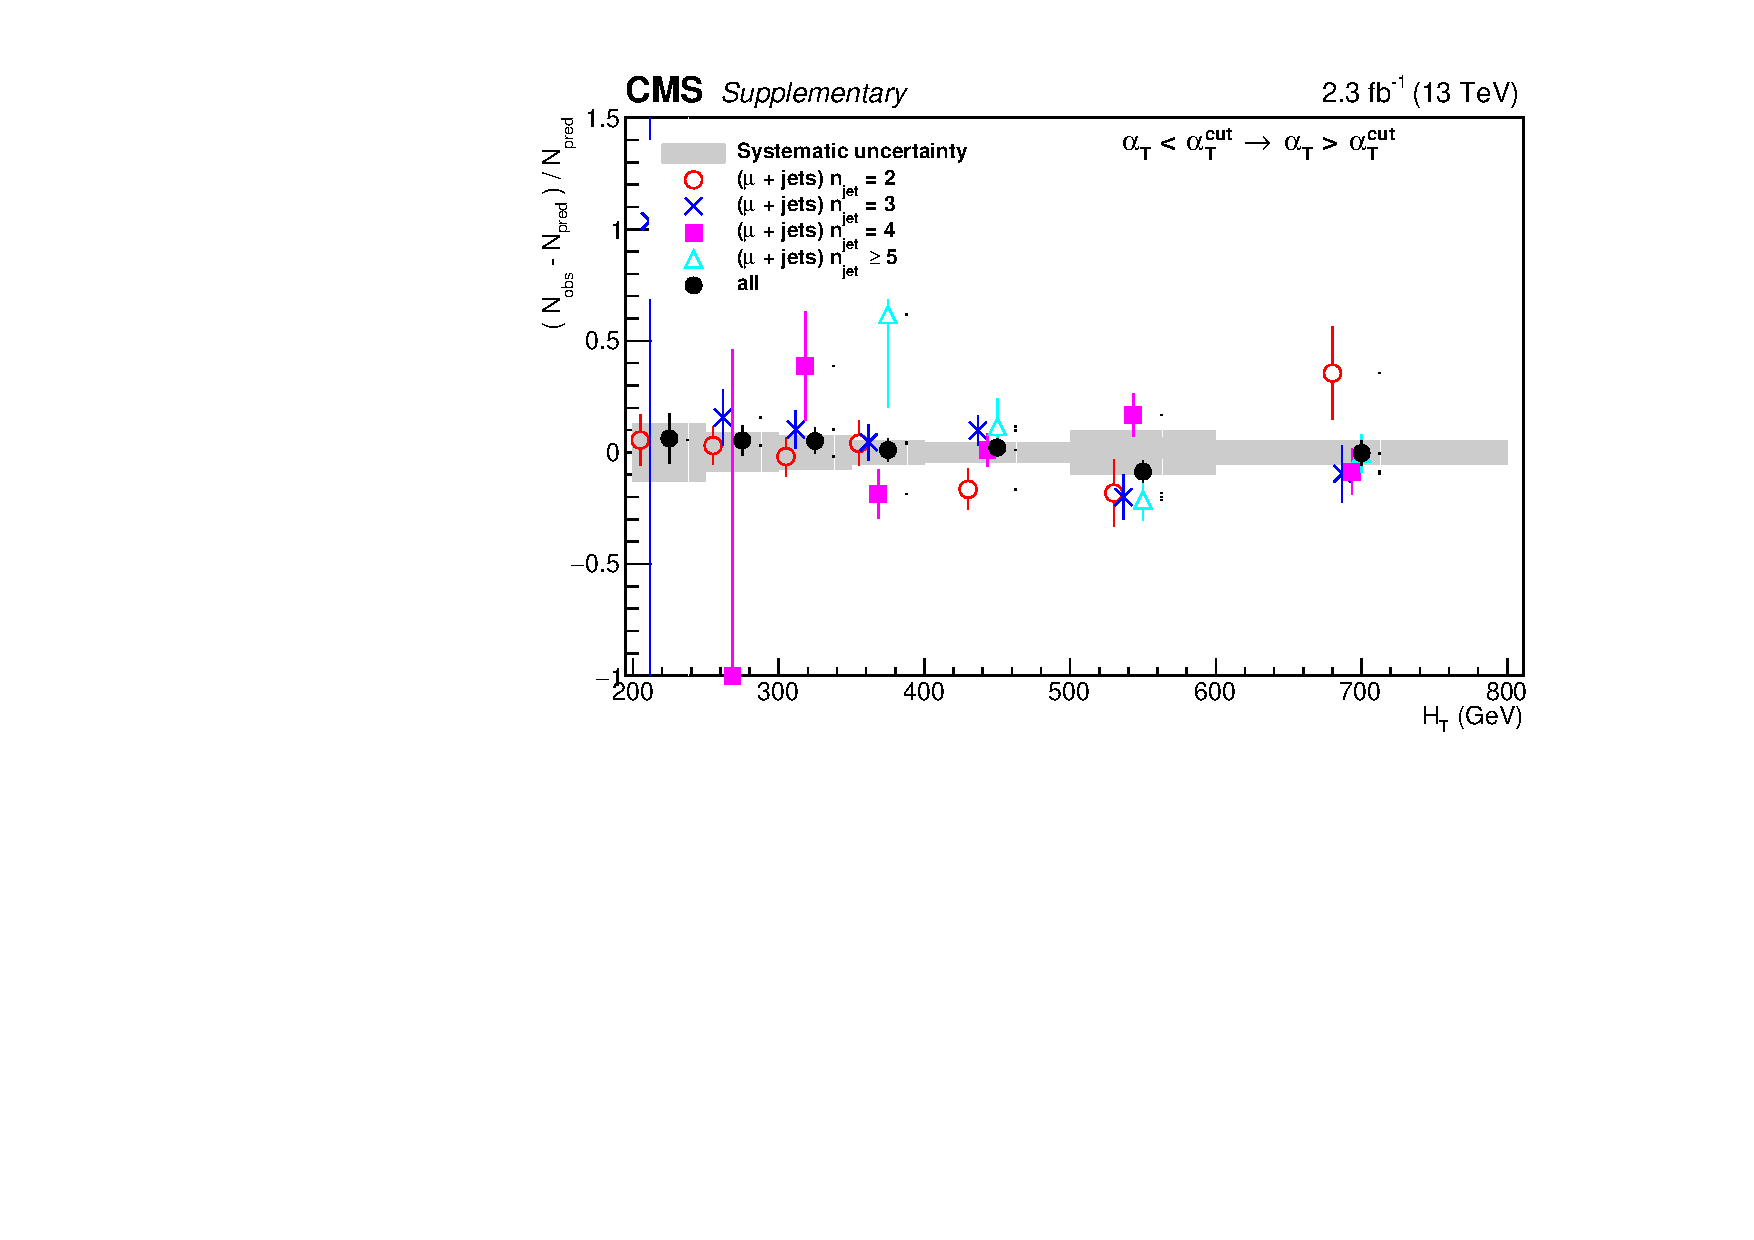
\includegraphics[width=0.48\textwidth]{Supplementary/alphaTsym__noFit_aux} ~~
     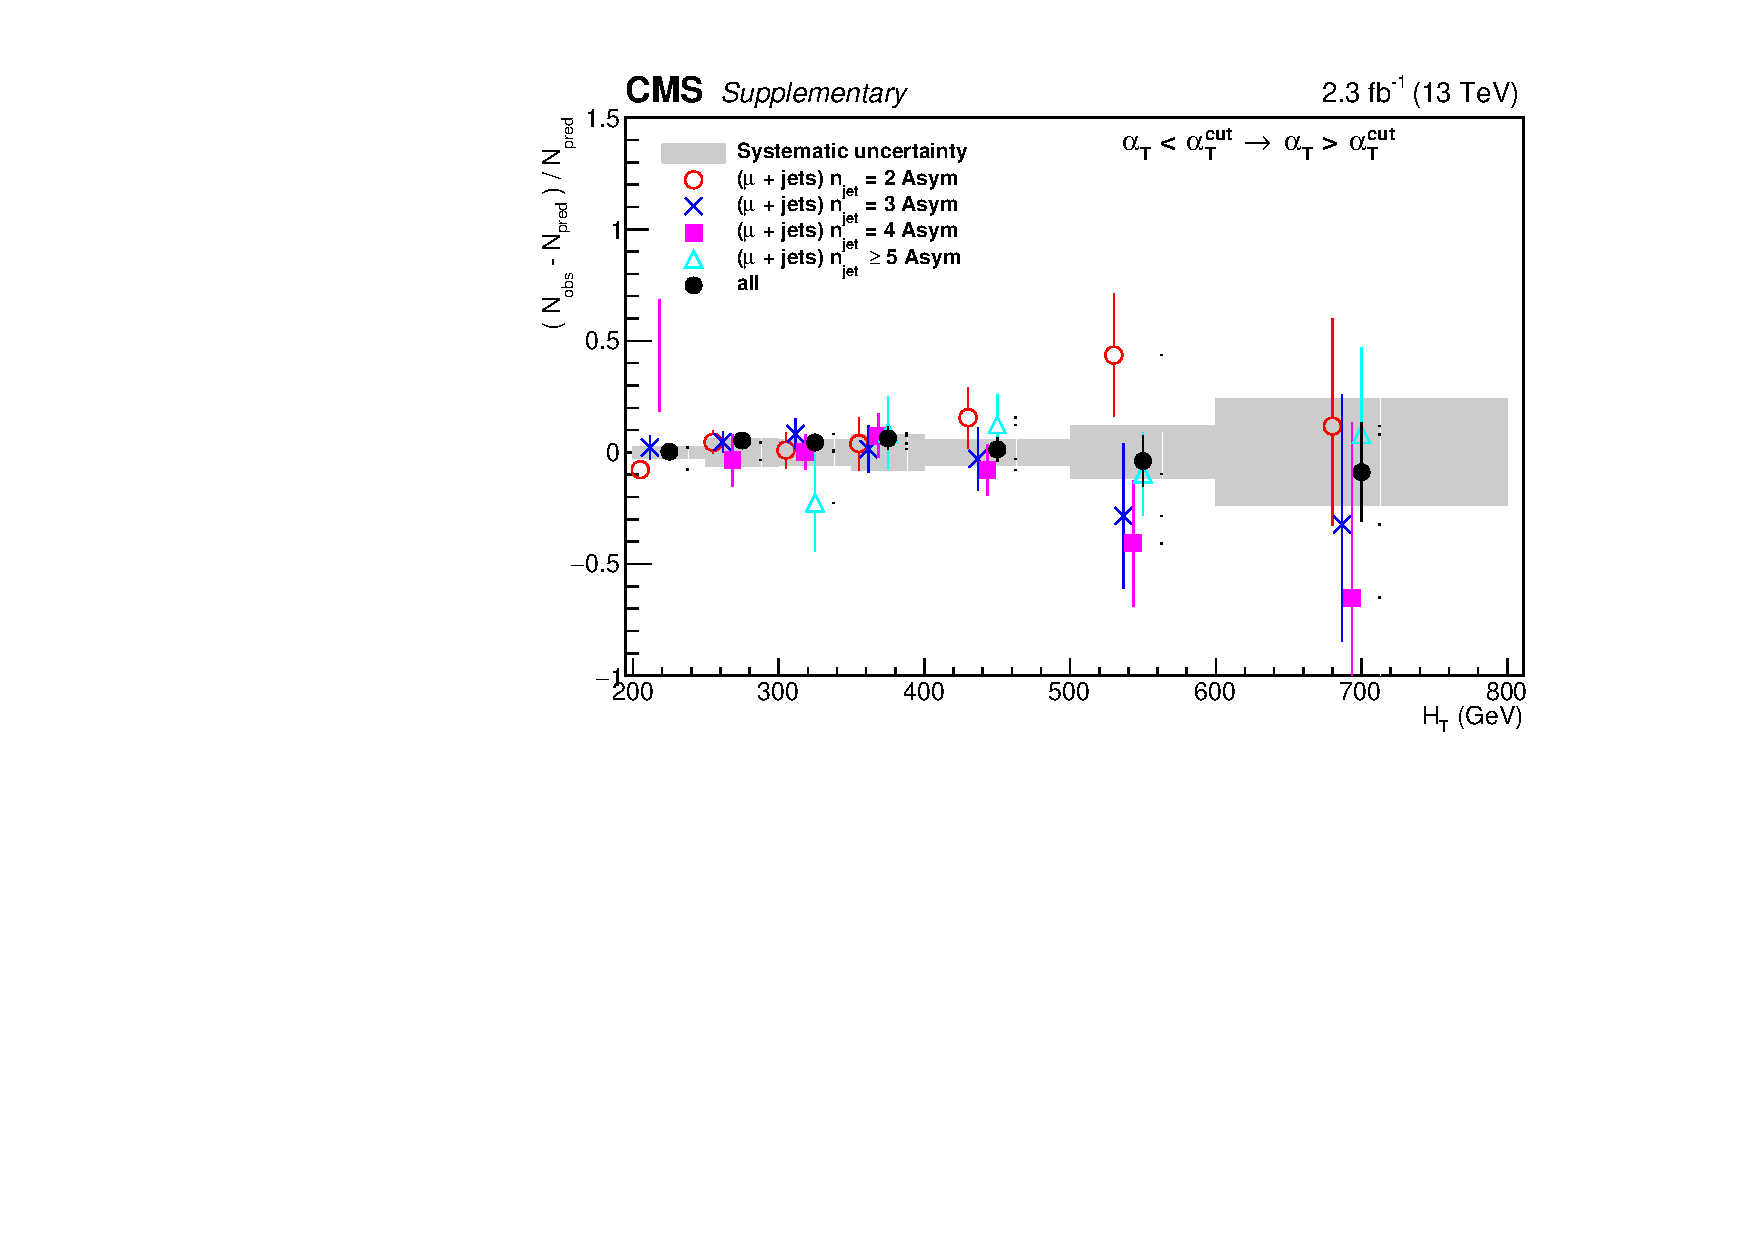
\includegraphics[width=0.48\textwidth]{Supplementary/alphaTasym__noFit_aux}
  \end{center}
\end{figure}

\begin{figure}[tbhp]
    \caption{ 
  Data-derived test of the modelling of the Z/W ratio for the symmetric (left) and asymmetric (right) jet categories. 
  In this test, the data yield in the \mmj sample ($N_{\mathrm{obs}}$) 
  is compared with the prediction obtained from the \mj sample multiplied by the corresponding 
  transfer factor computed in simulation ($N_{\mathrm{pred}}$). 
  A systematic uncertainty (grey band) is derived, as a function of $H_{\mathrm{T}}$ and separately for symmetric and asymmetric categories, 
  to cover the non-closure. 
    \label{fig:CT-ZWratio} }
  \begin{center}
     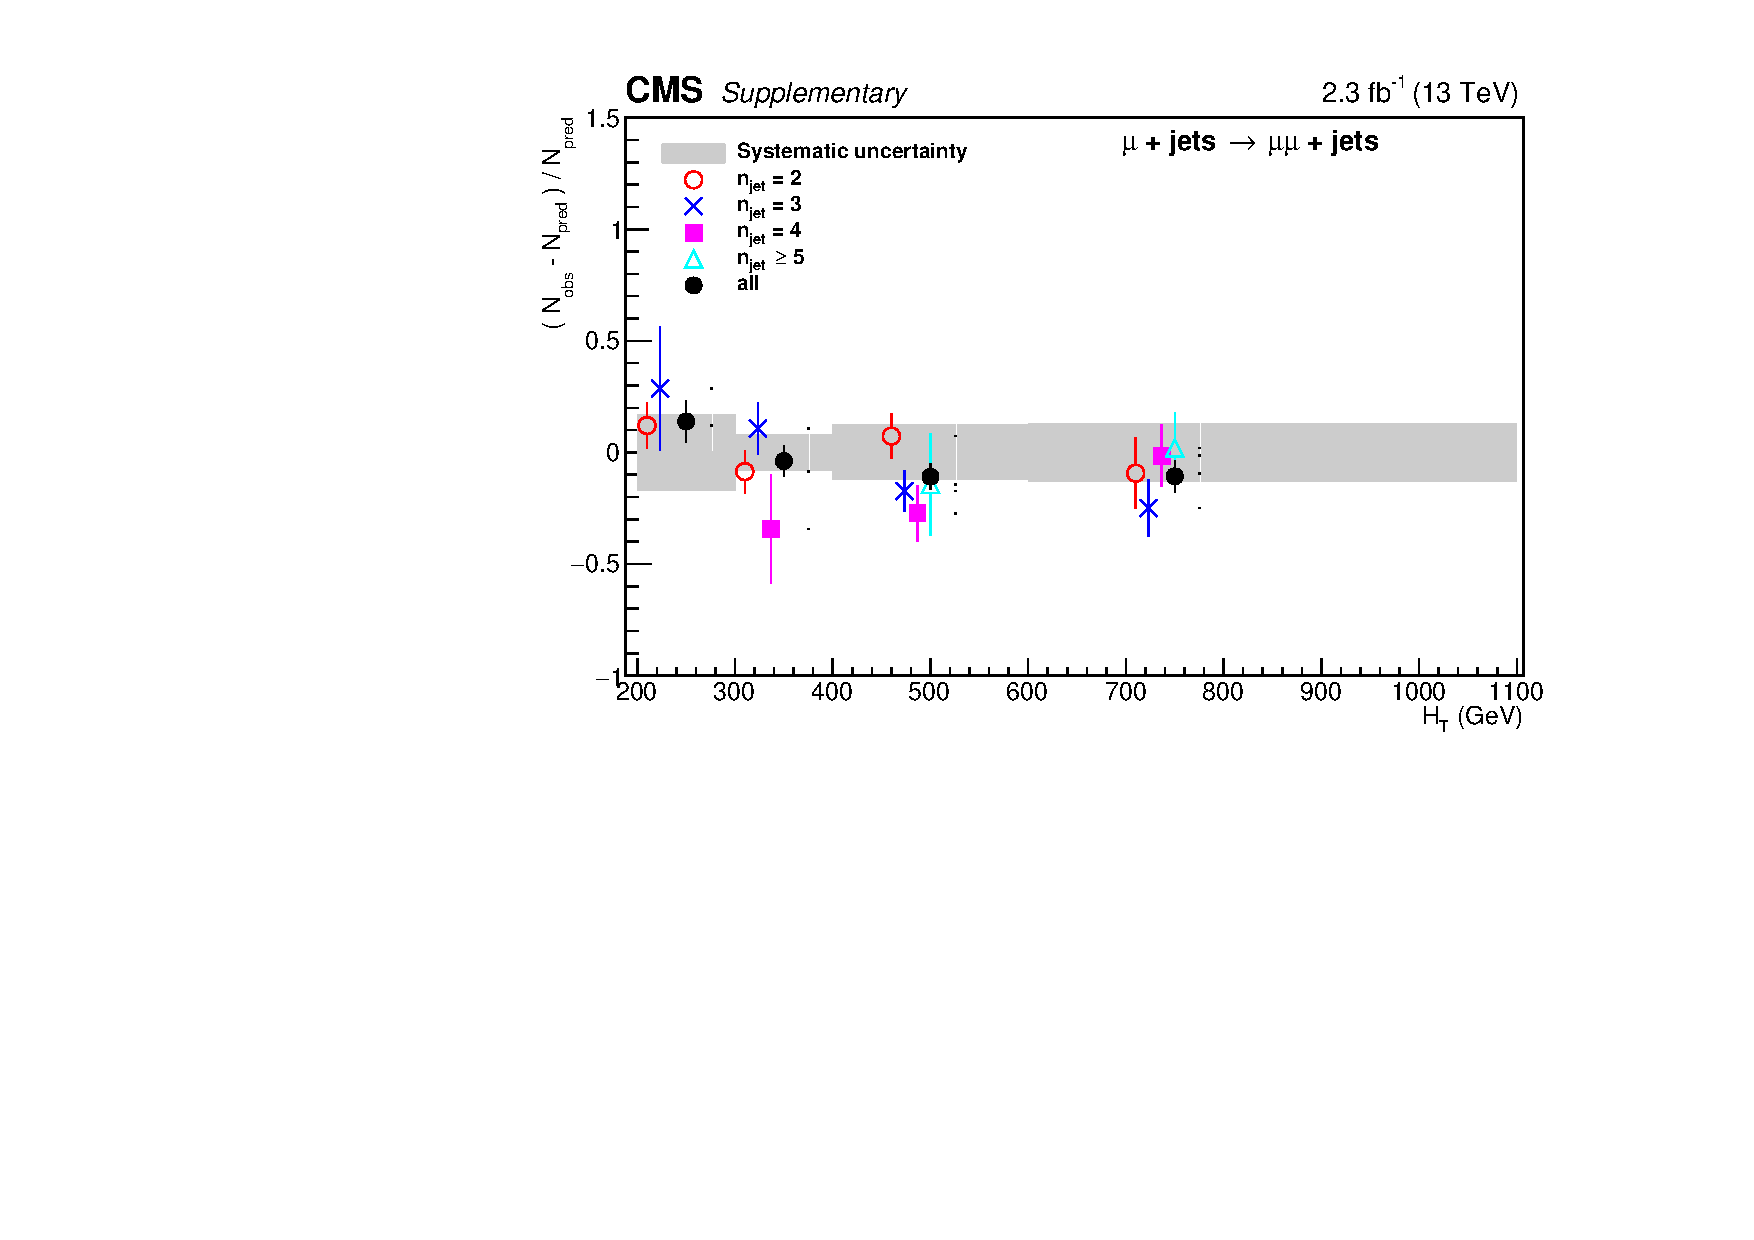
\includegraphics[width=0.48\textwidth]{Supplementary/mu_mumusym_half_noFit_aux} ~~
     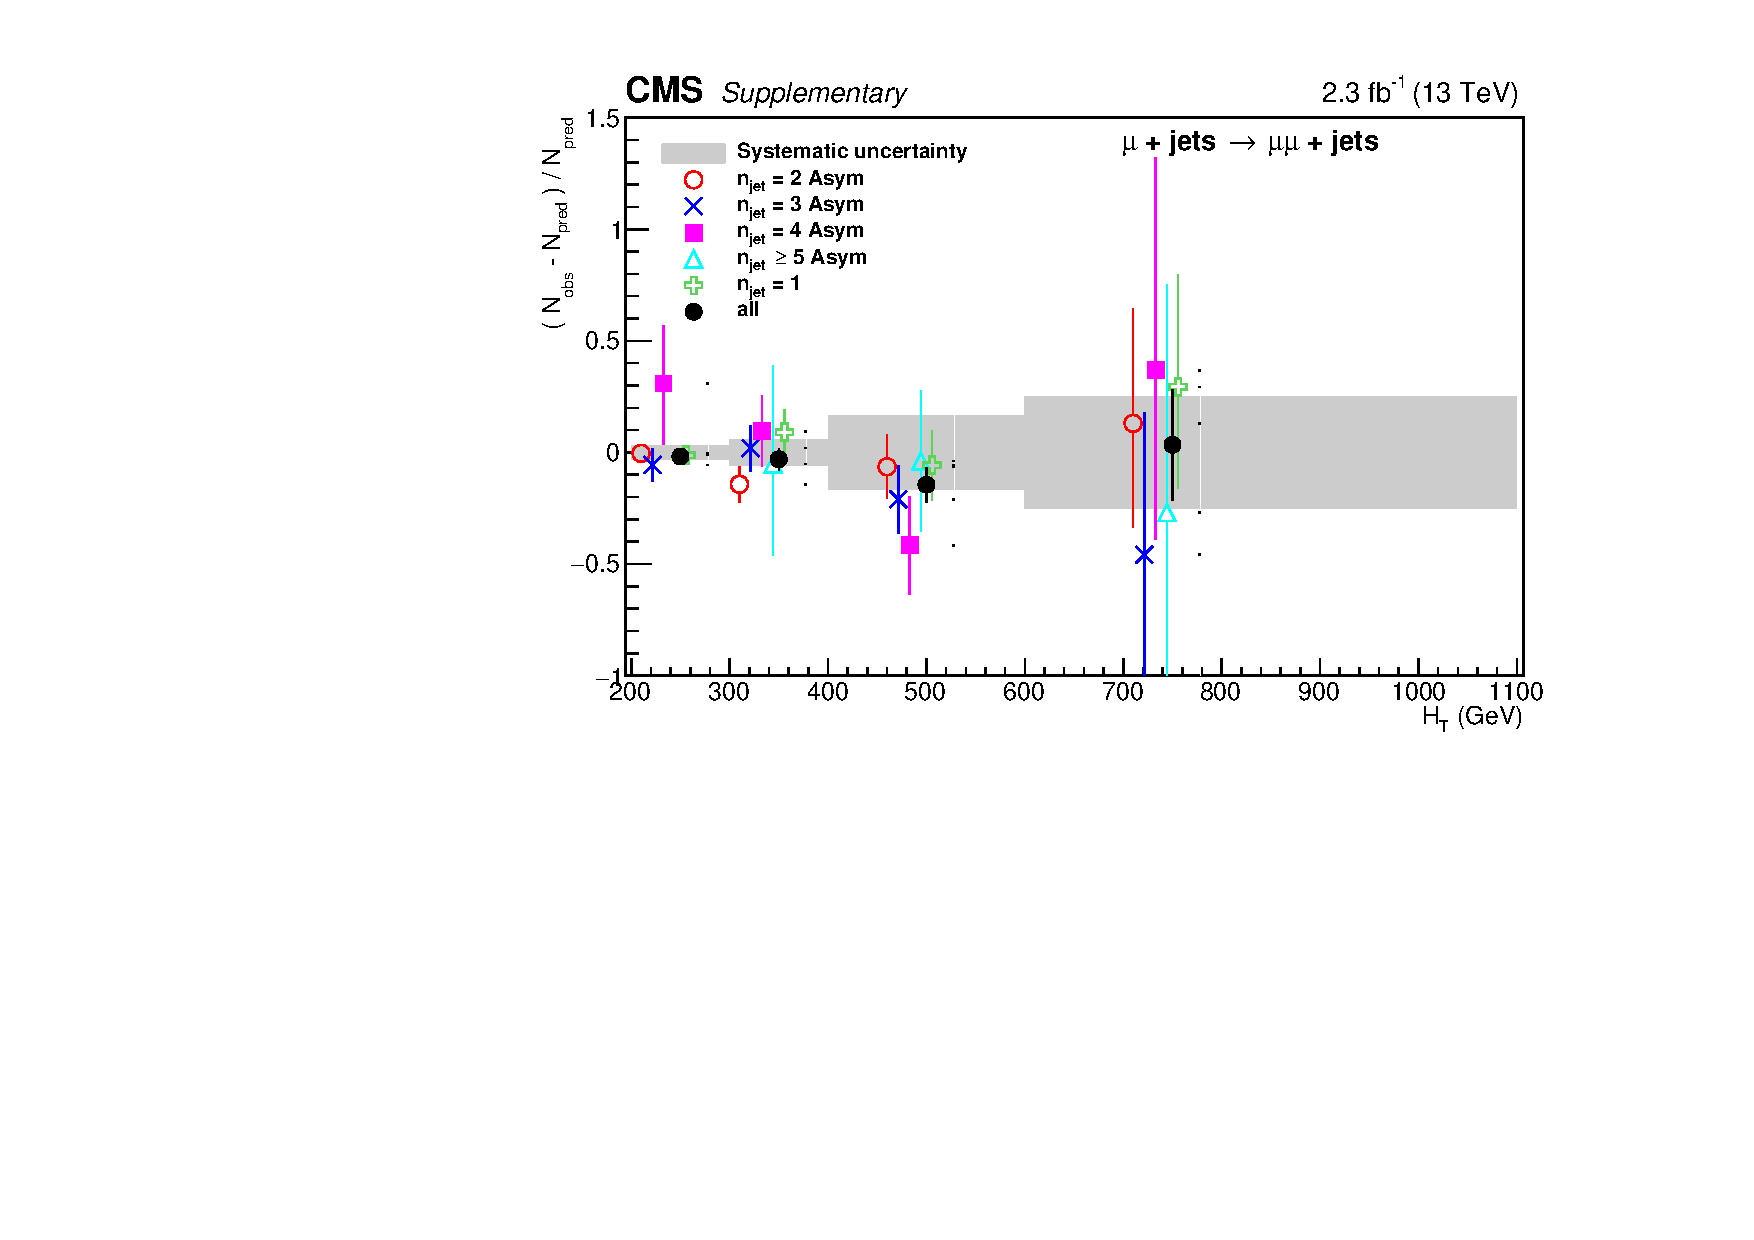
\includegraphics[width=0.48\textwidth]{Supplementary/mu_mumuasym_half_noFit_aux}
  \end{center}
\end{figure}





\clearpage
\begin{figure}[tbhp]
    \caption{ 
    Validation of the $H_{\mathrm{T}}^{miss}$ modelling in the MC, in bins of ($n_{\mathrm{jet}}$,$n_{\mathrm{b}}$,$H_{\mathrm{T}}$), for 
    $\gamma+\mathrm{jets}$,
    $n_{\mathrm{jet}}=2,n_{\mathrm{b}}=0,600<H_{\mathrm{T}}<800 \,
    \mathrm{GeV}$ (upper left),
    $\gamma+\mathrm{jets}$,
    $n_{\mathrm{jet}}=4,n_{\mathrm{b}}=1,600<H_{\mathrm{T}}<800 \,
    \mathrm{GeV}$ (upper right),
    $\mu+\mathrm{jets}$,
    $n_{\mathrm{jet}}^{asym}\geq5,n_{\mathrm{b}}=2,350<H_{\mathrm{T}}<400
    \, \mathrm{GeV}$ (middle left),
    $\mu+\mathrm{jets}$,
    $n_{\mathrm{jet}}\geq5,n_{\mathrm{b}}=0,H_{\mathrm{T}}>800 \,
    \mathrm{GeV}$ (middle right),
    $\mu\mu+\mathrm{jets}$,
    $n_{\mathrm{jet}}^{asym}=3,n_{\mathrm{b}}=0,200<H_{\mathrm{T}}<250
    \, \mathrm{GeV}$ (lower left),
    $\mu\mu+\mathrm{jets}$,
    $n_{\mathrm{jet}}=2,n_{\mathrm{b}}=0,400<H_{\mathrm{T}}<500 \,
    \mathrm{GeV}$ (lower right).
    The data/MC ratio is fitted with constant and linear functions to spot for possible 
    trends and the result of these fits are shown in the plot. The best fit value of the linear function and its uncertainty are propagated 
    to assign shape systematic uncertainty in each ($n_{\mathrm{jet}}$,$n_{\mathrm{b}}$,$H_{\mathrm{T}}$) category. 
    \label{fig:mht-validation} }
  \begin{center}
    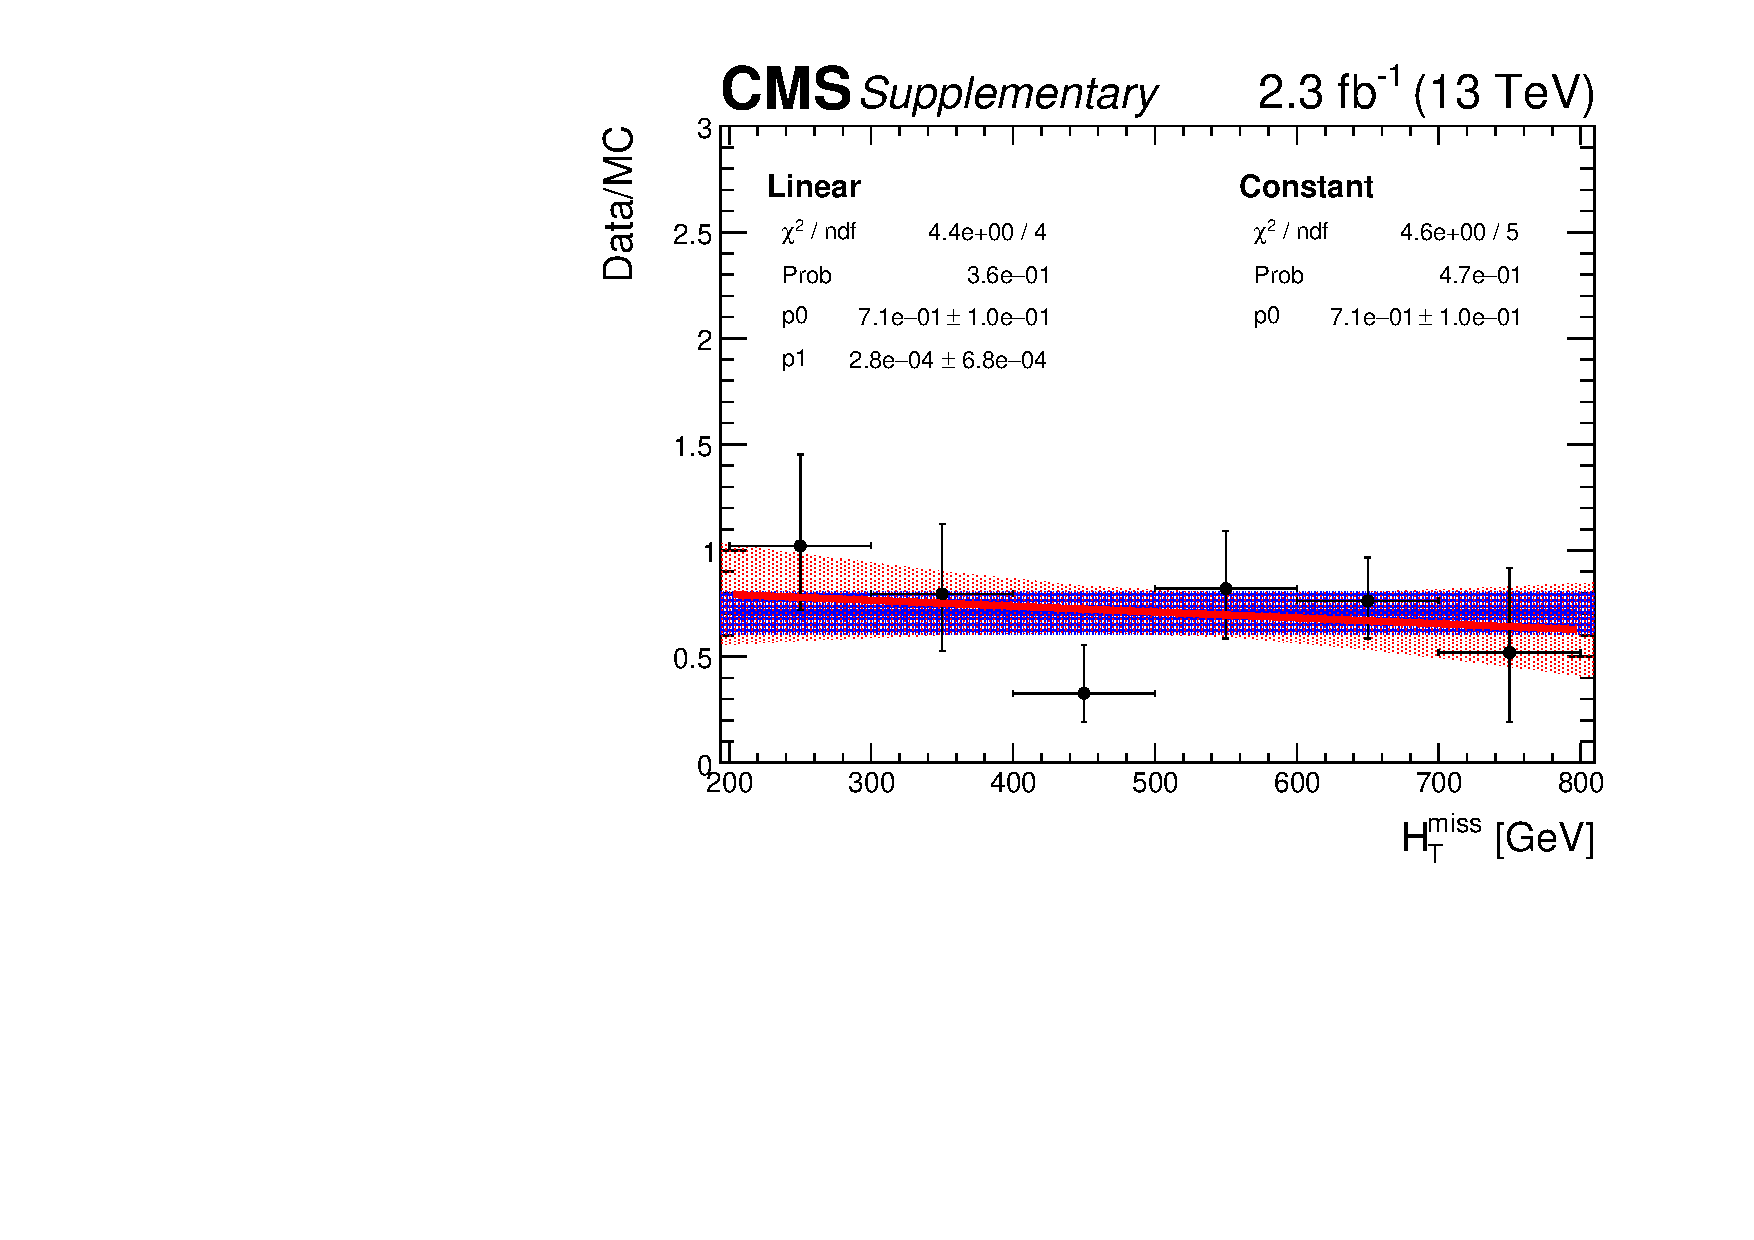
\includegraphics[width=0.45\textwidth]{Supplementary/mht_eq0b_eq2j_ht_600_800_SinglePhoton_Graph_aux}  ~~
    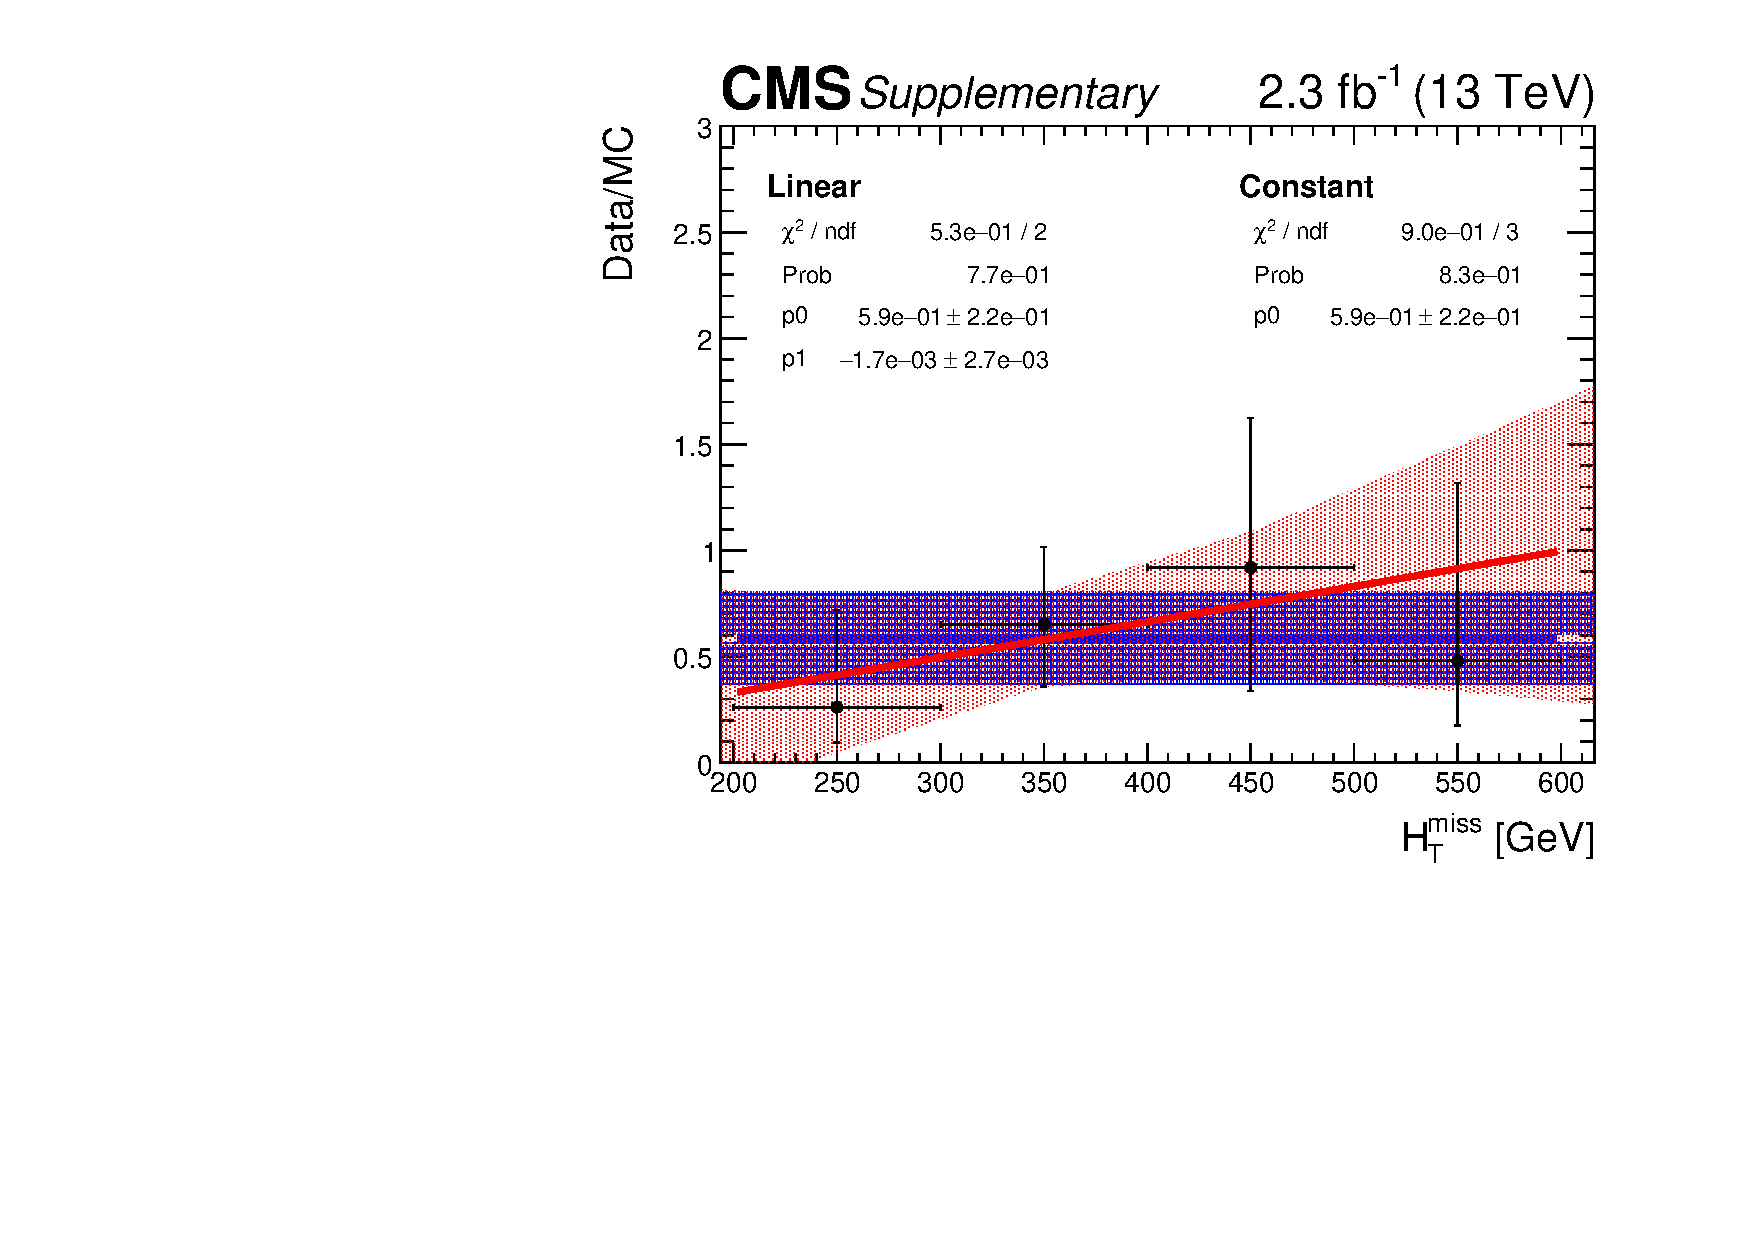
\includegraphics[width=0.45\textwidth]{Supplementary/mht_eq1b_eq4j_ht_600_800_SinglePhoton_Graph_aux}  \\
    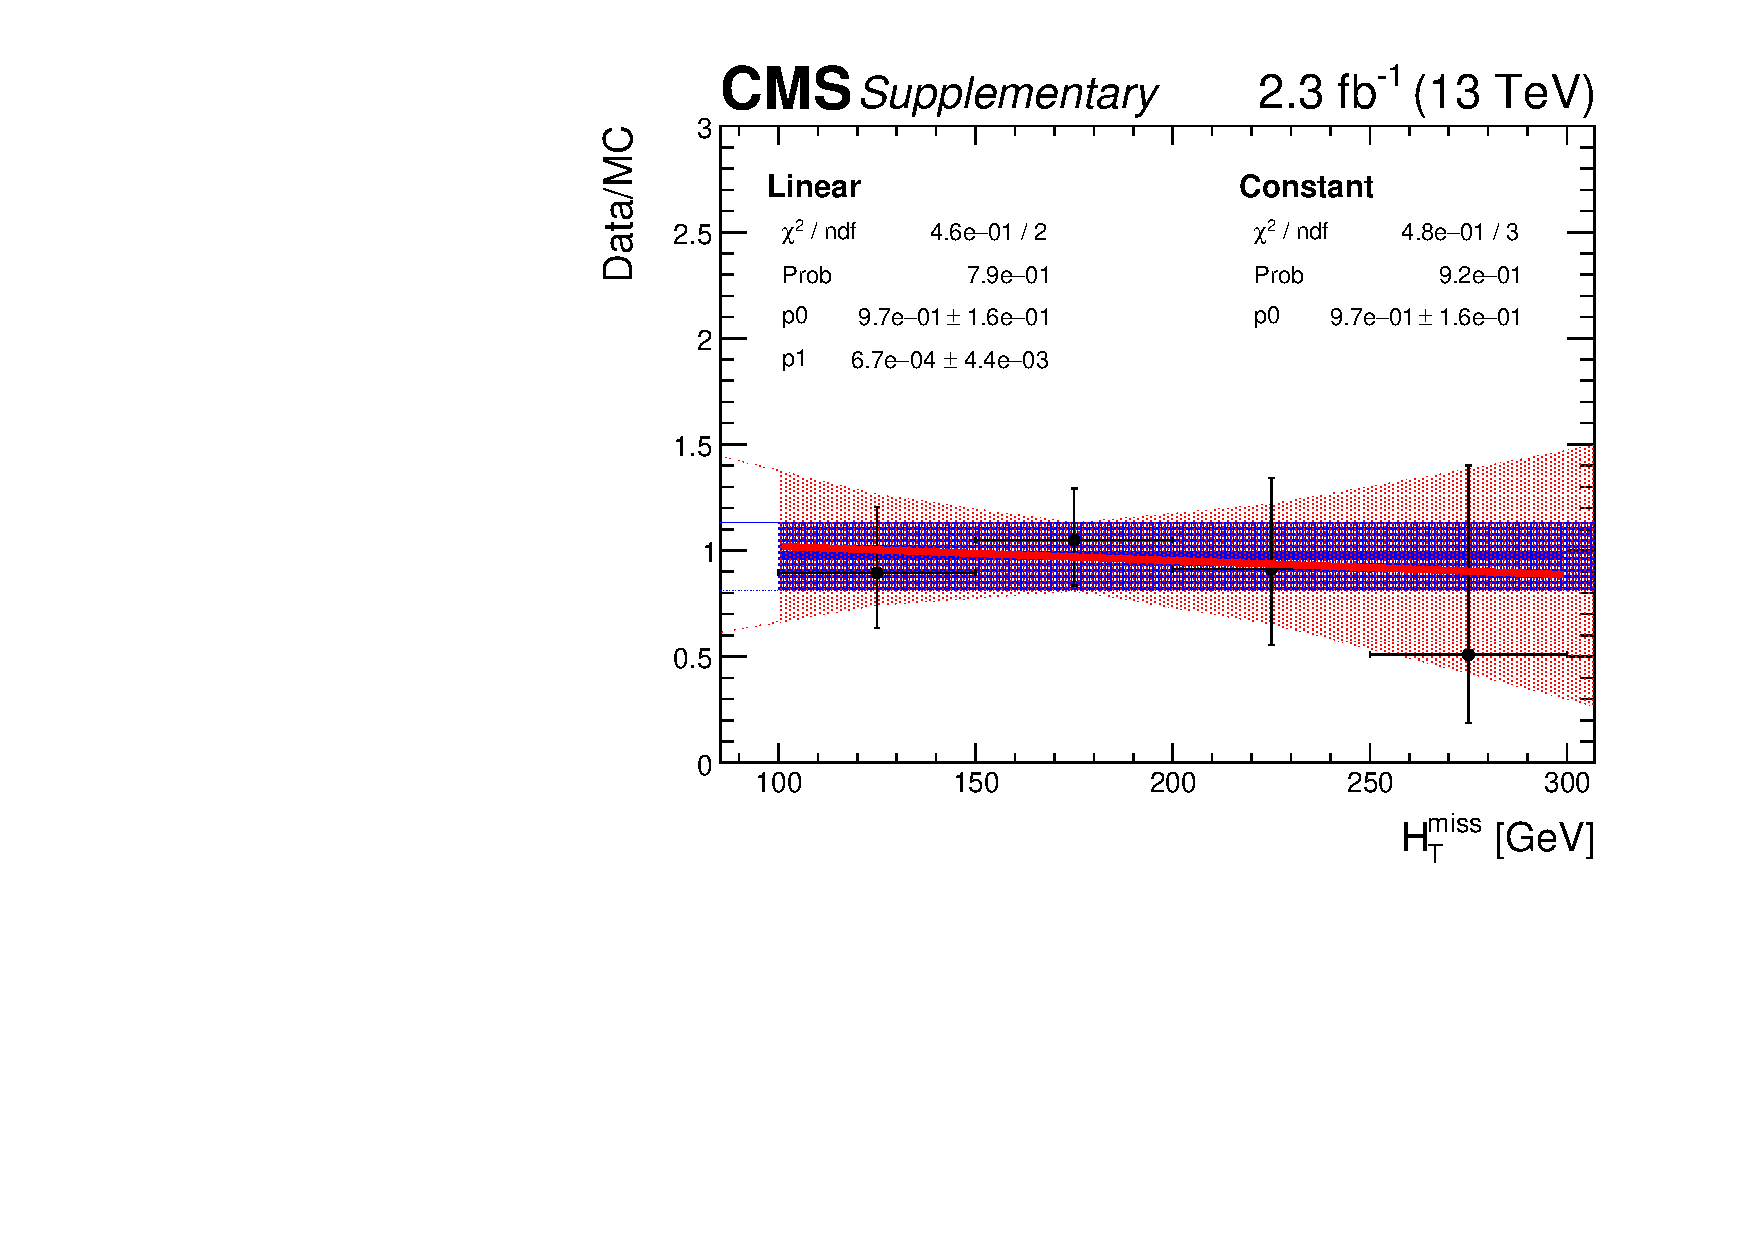
\includegraphics[width=0.45\textwidth]{Supplementary/mht_eq2b_ge5a_ht_350_400_SingleMu_Graph_aux}  ~~
    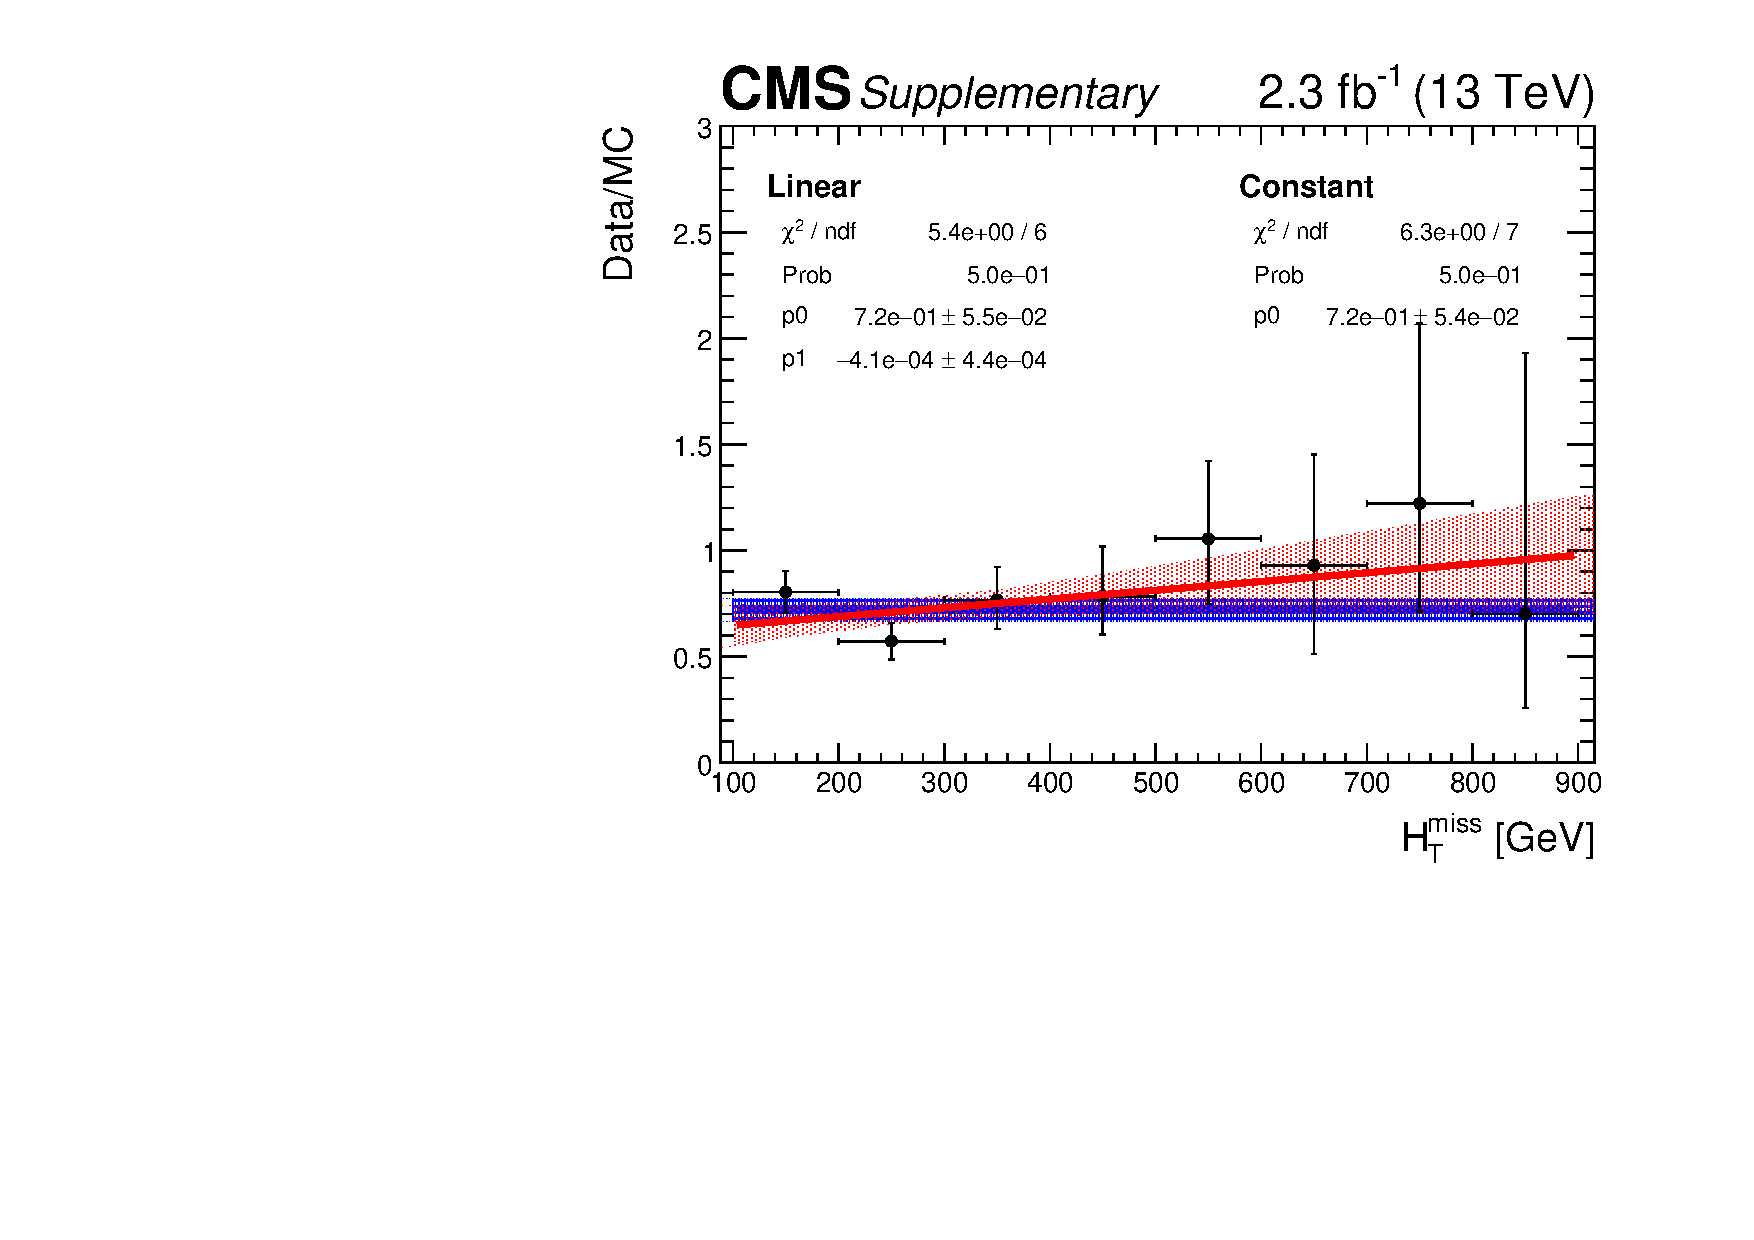
\includegraphics[width=0.45\textwidth]{Supplementary/mht_eq0b_ge5j_ht_800_Inf_SingleMu_Graph_aux}  \\
    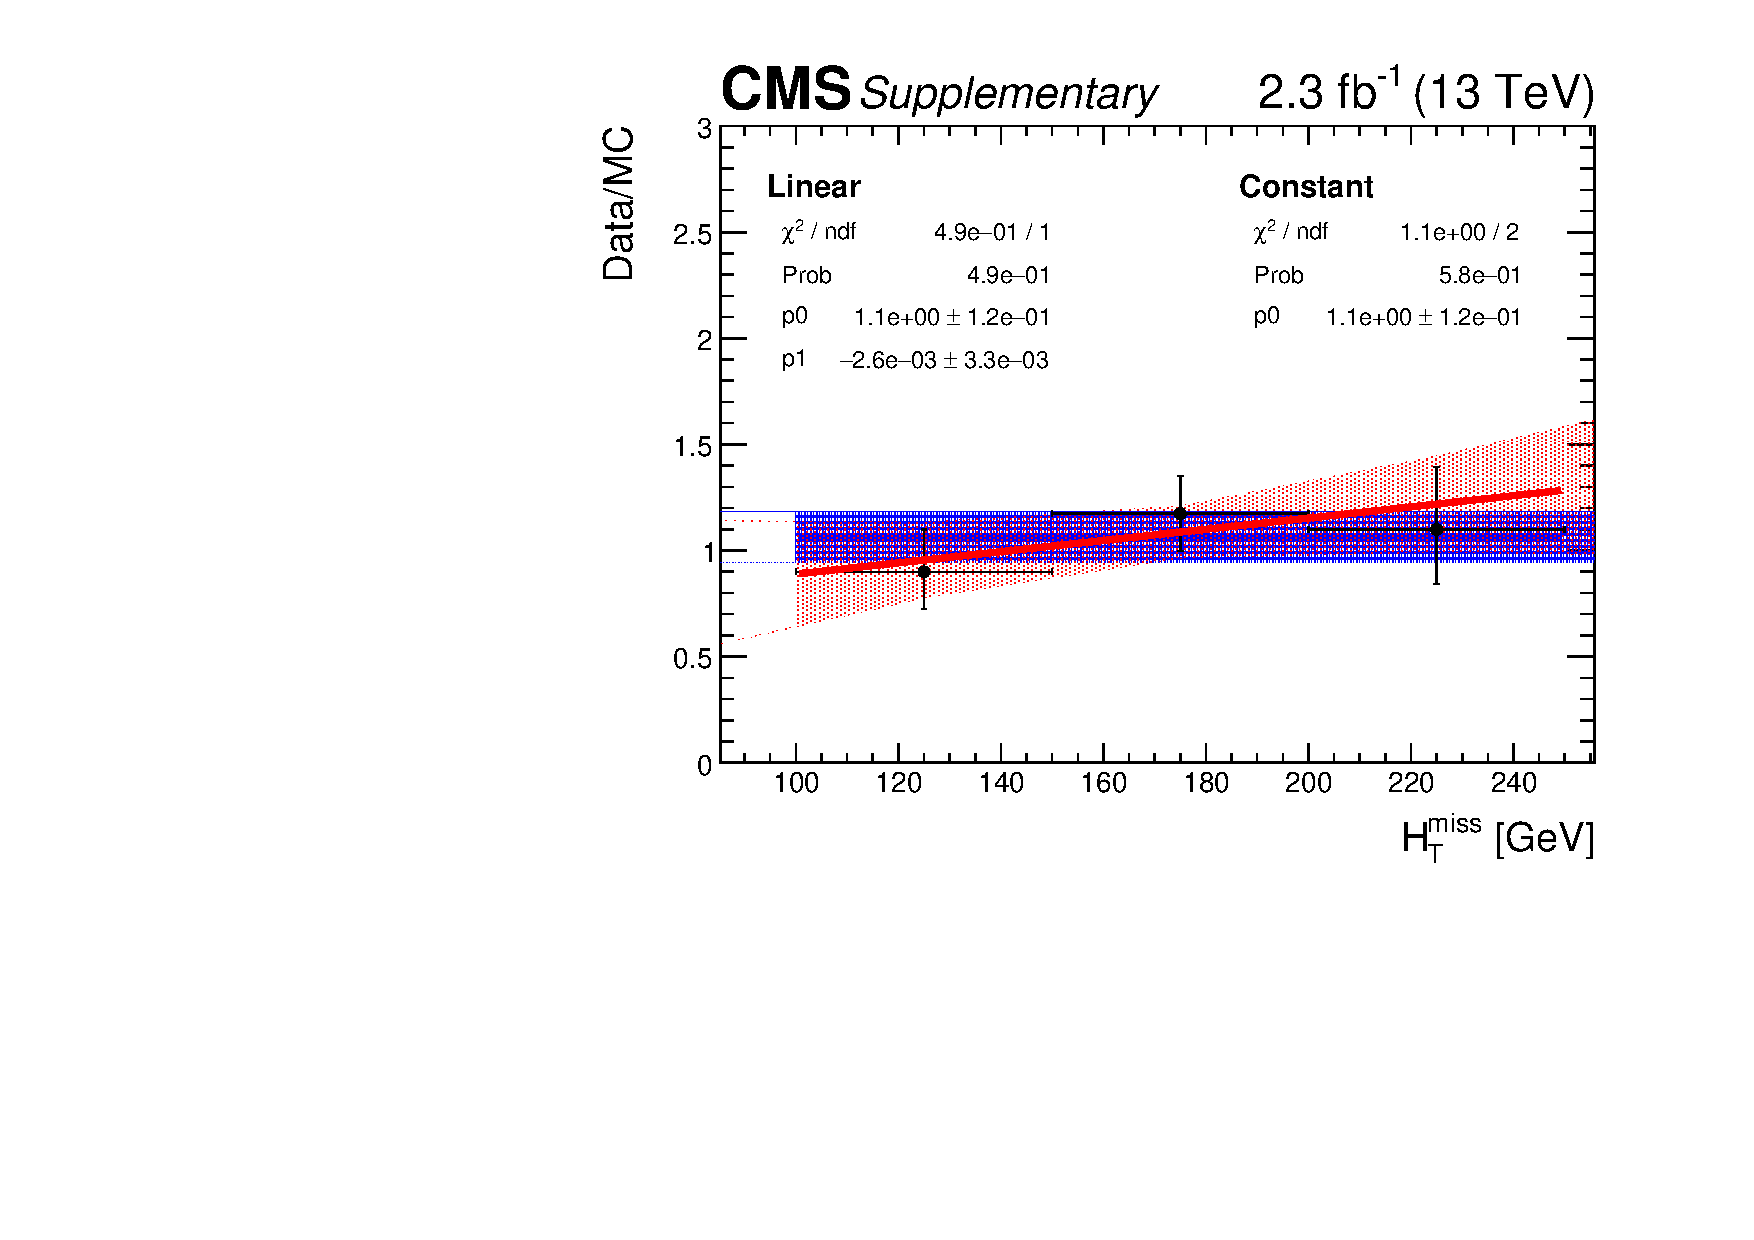
\includegraphics[width=0.45\textwidth]{Supplementary/mht_eq0b_eq3a_ht_200_250_DoubleMu_Graph_aux}  ~~
    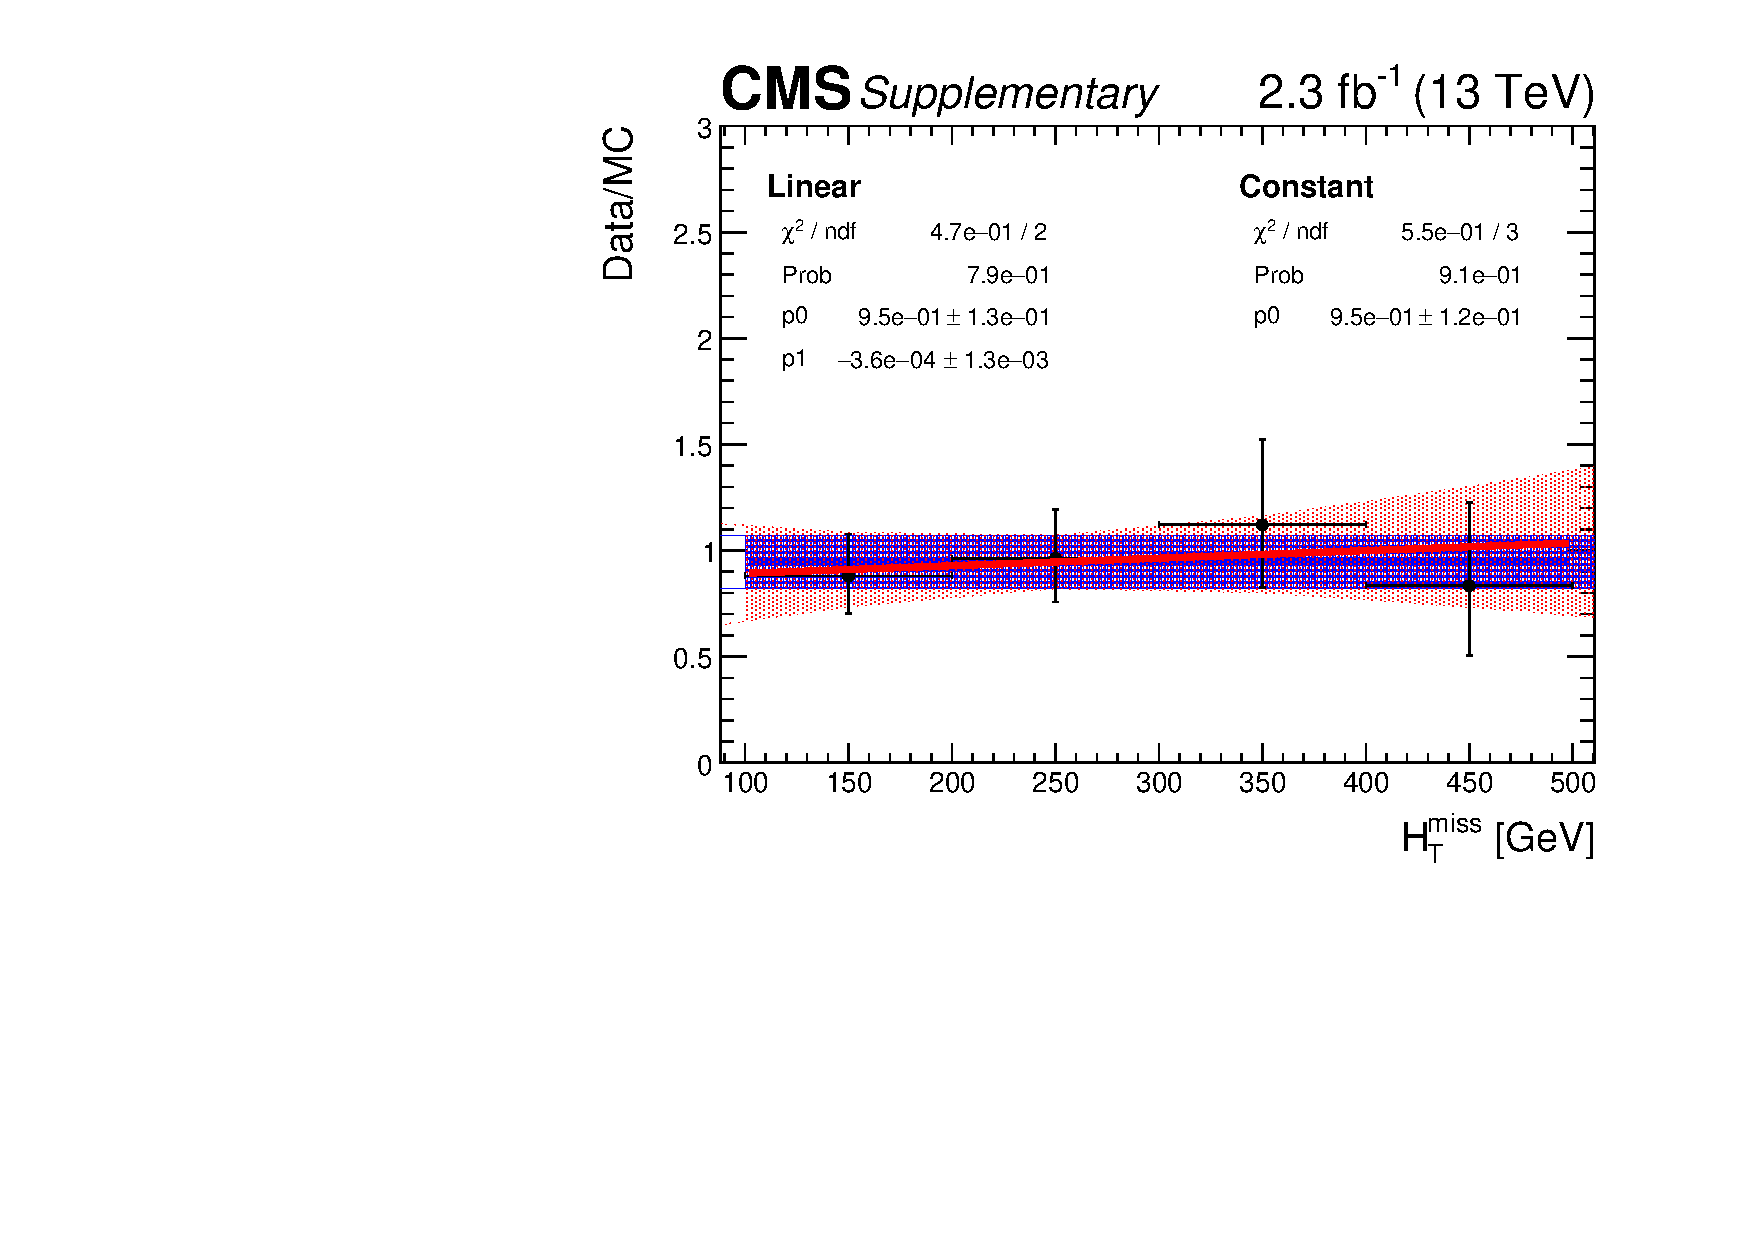
\includegraphics[width=0.45\textwidth]{Supplementary/mht_eq0b_eq2j_ht_400_500_DoubleMu_Graph_aux}  \\
  \end{center}
\end{figure}


\clearpage
\begin{figure}[tbhp]
    \caption{ 
    Histogram templates in the $H_{\mathrm{T}}^{miss}$ dimension, for $n_{\mathrm{jet}} \geq 5$, $n_{\mathrm{b}} \geq 3$, $H_{\mathrm{T}} > 800$ GeV (a) and 
    $n_{\mathrm{jet}} \geq 5$, $n_{\mathrm{b}} = 2$, $H_{\mathrm{T}} > 800$ GeV (b). 
    The data (black points) are compared with the total pre-fit background expectation (blue) and its total uncertainty (grey band). 
    The breakdown for each background component is also shown. 
    In the bottom part of the plot the pull for each bin is shown, defined as $(\mathrm{data}-\mathrm{SM total})/\sigma_{bkg}$, where $\sigma_{bkg}=\sqrt{\sigma^{2}_{syst.}+\sigma^{2}_{stat.}}$. 
    Examples of benchmark models are also shown. \label{fig:mht-templates} }
  \begin{center}
    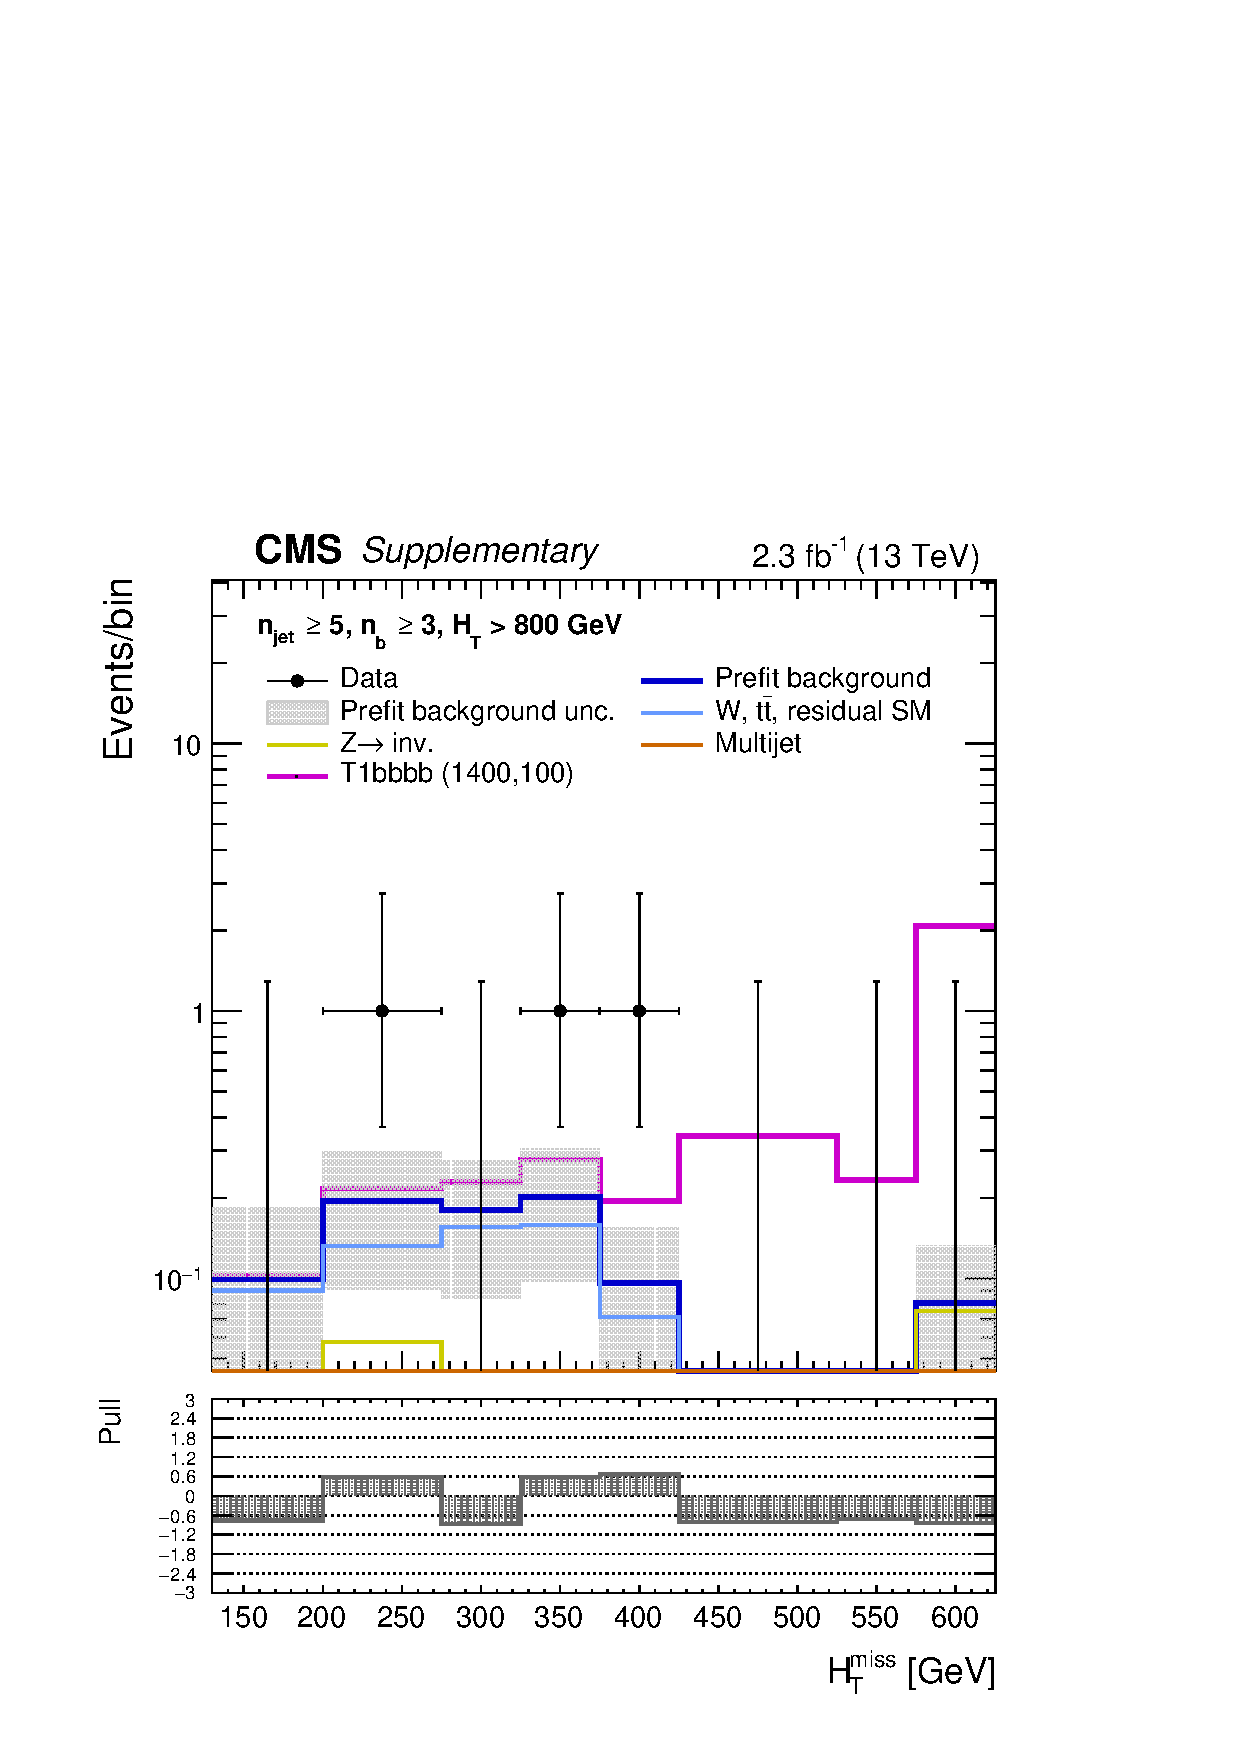
\includegraphics[width=0.45\textwidth]{Supplementary/postFitShape_ge3b_ge5j_800_Inf_prefit_T1bbbb_1400_100_aux} ~~
    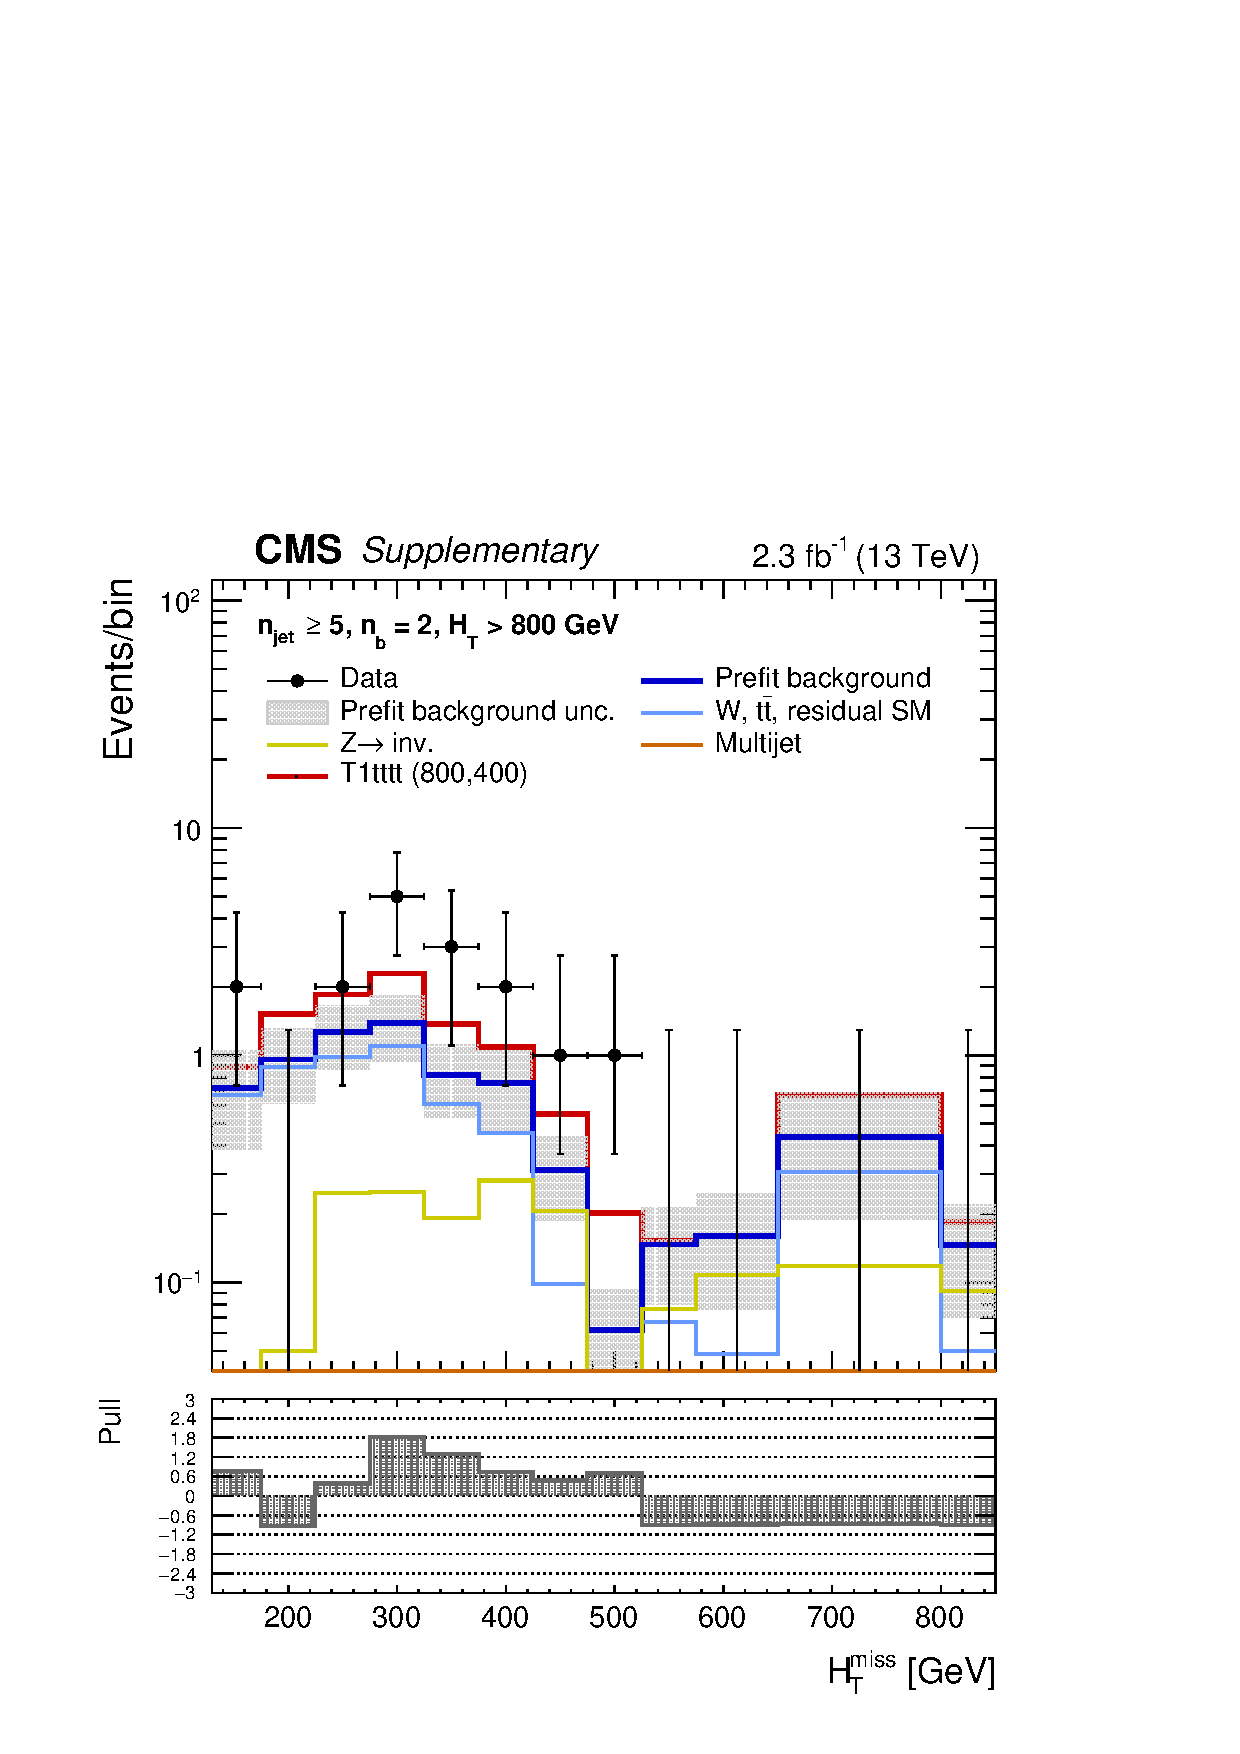
\includegraphics[width=0.45\textwidth]{Supplementary/postFitShape_eq2b_ge5j_800_Inf_prefit_T1tttt_800_400_aux} \\
  \end{center}
\end{figure}


\clearpage
\begin{figure*}[t]
  \begin{center}
    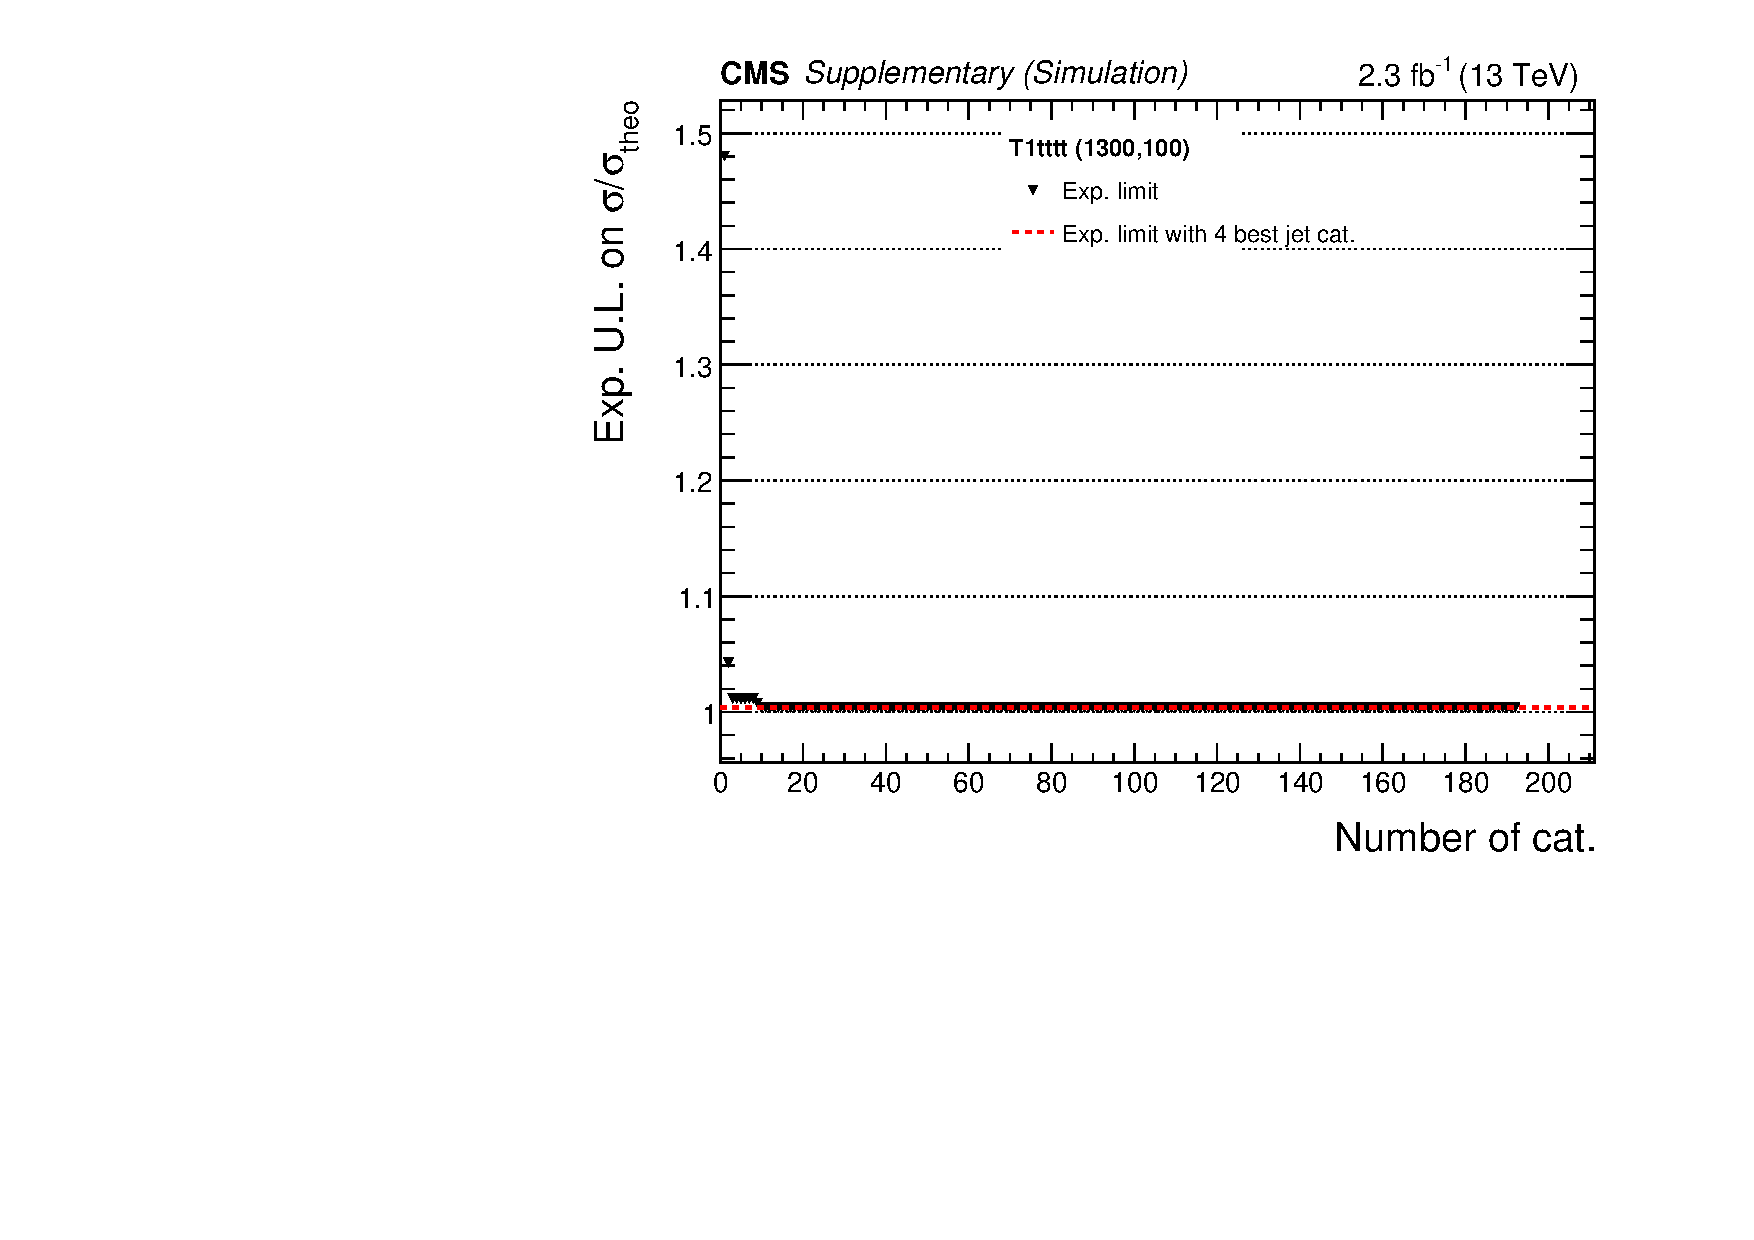
\includegraphics[width=0.49\textwidth]{Supplementary/expVsCat_SMS-T1tttt_mGluino-1300_mLSP-100_25ns_aux} \, 
    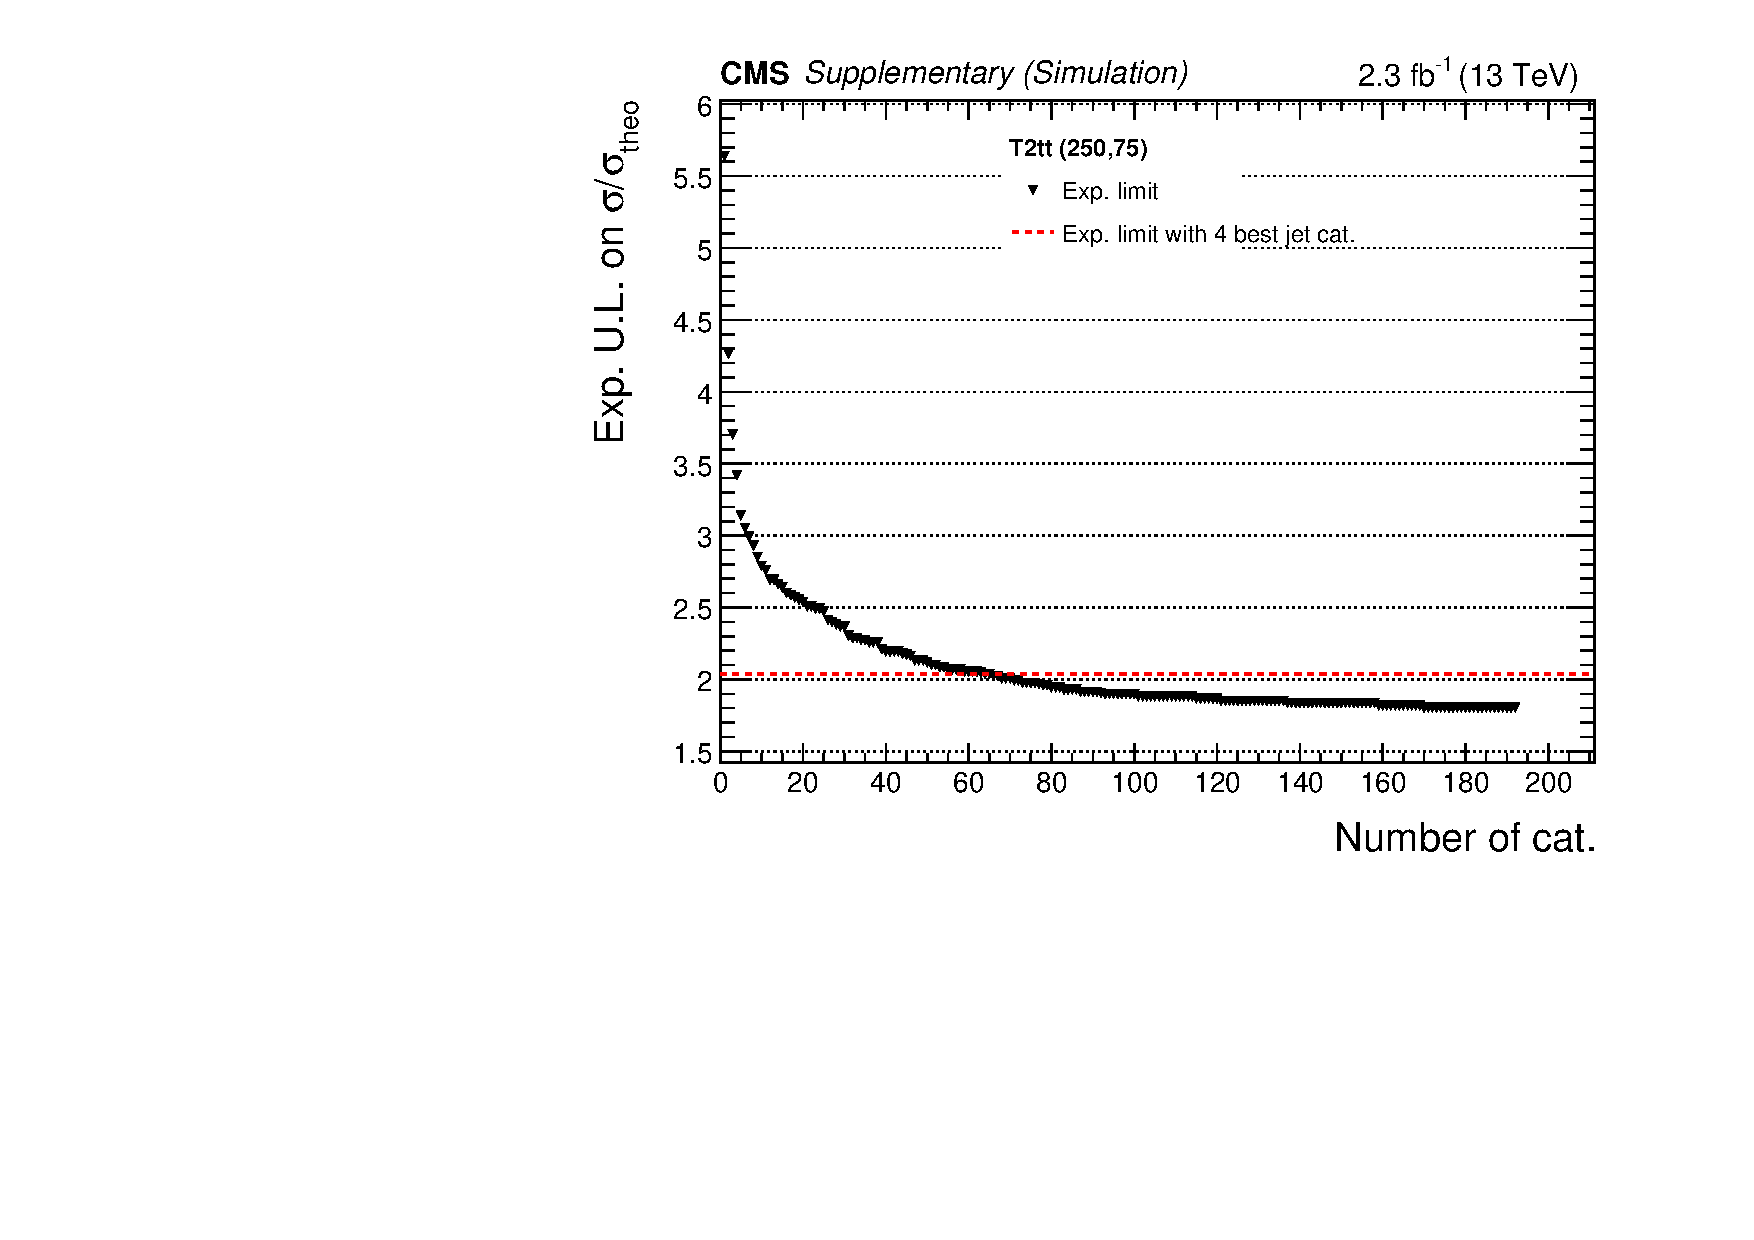
\includegraphics[width=0.49\textwidth]{Supplementary/expVsCat_SMS-T2tt_mStop-250_mLSP-75_25ns_aux} \,     
  \end{center}
  \caption{
  The expected upper limit (black points) on the signal strength
  $\sigma / \sigma_{\mathrm{theo}}$ as a function of the number of
  ($n_{\mathrm{jet}}$, $n_{\mathrm{b}}$, $H_{\mathrm{T}}$) categories
  included in the fit, where the categories are ranked according to
  the expected exclusion, for one T1tttt (T2tt) benchmark point on the
  left (right) plot. The red dashed line is the expected upper limit
  determined from the four most sensitive jet categories, as is done
  for the final limit calculation in this analysis. For the purpose of
  this test the MC statistical uncertainty in each bin has not been
  considered. The study depicted by the black points has to be
  regarded only as an approximate indication of the number of
  categories contributing to the exclusion, as some of the
  correlations may be neglected. 
  \label{fig:sensitivityVsCat}}
\end{figure*}


\clearpage
\begin{table}[h!] 
  \scriptsize
  \caption{ 
  Signal yield, background expectation and data observation for the 10
  most excluding
  ($n_{\mathrm{jet}}$,$n_{\mathrm{b}}$,$H_{\mathrm{T}}$) category for
  T1bbbb benchmark models.  
  Expected and observed upper limits on the signal strength
  $r=\sigma/\sigma_{\mathrm{theo}}$ are also shown  
  for each individual bin and for the 4 most excluding
  $n_{\mathrm{jet}}$ categories combined (with all the
  $n_{\mathrm{b}}$,$H_{\mathrm{T}}$ bin with each category). 
  It should be kept in mind that in the analysis jet categories are
  always considered with all their $n_{\mathrm{b}}$,$H_{\mathrm{T}}$
  bins  
  combined, in order to preserve the correlation of the systematic
  uncertainties.  
  Therefore the individual-bin limits shown in this table have to be
  regarded only as an approximate indication  
  of the sensitivity of each bin, as some of the correlations may be
  neglected. 
  \label{tab:sigBenchmarksYields_T1bbbb}}
  \centering 
  \begin{tabular}{ lllllll } 
    \hline 
    Model & Analysis bin & Signal & Background & Data & Exp. U. L. & Obs. U. L. \\ \hline
\multirow{10}{*}{\parbox[t]{2cm}{T1bbbb (1500,100)\\exp.: $r<0.81$\\obs.: $r<0.79$}}
 & $n_{\mathrm{jet}} \geq5j,n_{\mathrm{b}} \geq3$, $H_{\mathrm{T}} > 800 \, \mathrm{GeV}$ & 1.6 & $0.9 \pm 0.3 \mathrm{(syst.)} ^{+2.3}_{-1.9} \mathrm{(stat.)}$ & 3 & $r < 1.5$ & $r < 1.7$\\ 
 & $n_{\mathrm{jet}} \geq5j,n_{\mathrm{b}} =2$, $H_{\mathrm{T}} > 800 \, \mathrm{GeV}$ & 1.8 & $7.2 \pm 2.2 \mathrm{(syst.)} ^{+4.8}_{-3.7} \mathrm{(stat.)}$ & 16 & $r < 2.0$ & $r < 2.3$\\ 
 & $n_{\mathrm{jet}} \geq5j,n_{\mathrm{b}} =1$, $H_{\mathrm{T}} > 800 \, \mathrm{GeV}$ & 1.2 & $24.3 \pm 6.4 \mathrm{(syst.)} ^{+5.3}_{-4.7} \mathrm{(stat.)}$ & 21 & $r < 4.8$ & $r < 4.9$\\ 
 & $n_{\mathrm{jet}} =4j,n_{\mathrm{b}} \geq3$, $H_{\mathrm{T}} > 800 \, \mathrm{GeV}$ & 0.5 & $0.1 \pm 0.0 \mathrm{(syst.)} ^{+1.3}_{-0.0} \mathrm{(stat.)}$ & 0 & $r < 5.0$ & $r < 4.5$\\ 
 & $n_{\mathrm{jet}} =4j,n_{\mathrm{b}} =2$, $H_{\mathrm{T}} > 800 \, \mathrm{GeV}$ & 0.7 & $3.4 \pm 1.1 \mathrm{(syst.)} ^{+2.3}_{-1.3} \mathrm{(stat.)}$ & 2 & $r < 5.4$ & $r < 4.5$\\ 
 & $n_{\mathrm{jet}} =4j,n_{\mathrm{b}} =1$, $H_{\mathrm{T}} > 800 \, \mathrm{GeV}$ & 0.5 & $14.4 \pm 3.6 \mathrm{(syst.)} ^{+3.8}_{-3.2} \mathrm{(stat.)}$ & 10 & $r < 12.9$ & $r < 10.3$\\ 
 & $n_{\mathrm{jet}} =3j,n_{\mathrm{b}} =2$, $H_{\mathrm{T}} > 800 \, \mathrm{GeV}$ & 0.1 & $1.3 \pm 0.4 \mathrm{(syst.)} ^{+1.8}_{-0.6} \mathrm{(stat.)}$ & 1 & $r < 22.1$ & $r < 26.5$\\ 
 & $n_{\mathrm{jet}} =3j,n_{\mathrm{b}} =1$, $H_{\mathrm{T}} > 800 \, \mathrm{GeV}$ & 0.2 & $11.6 \pm 3.1 \mathrm{(syst.)} ^{+3.8}_{-3.2} \mathrm{(stat.)}$ & 10 & $r < 32.1$ & $r < 27.1$\\ 
 & $n_{\mathrm{jet}} \geq5j,n_{\mathrm{b}} =0$, $H_{\mathrm{T}} > 800 \, \mathrm{GeV}$ & 0.3 & $63.1 \pm 15.1 \mathrm{(syst.)} ^{+8.0}_{-8.0} \mathrm{(stat.)}$ & 64 & $r < 48.6$ & $r < 45.8$\\ 
 & $n_{\mathrm{jet}} =3j,n_{\mathrm{b}} \geq3$, $H_{\mathrm{T}} > 400 \, \mathrm{GeV}$ & 0.0 & $0.5 \pm 0.2 \mathrm{(syst.)} ^{+1.8}_{-0.6} \mathrm{(stat.)}$ & 1 & $r < 64.6$ & $r < 82.4$\\ \hline
\multirow{10}{*}{\parbox[t]{2cm}{T1bbbb (1000,800)\\exp.: $r<0.33$\\obs.: $r<0.32$}}
 & $n_{\mathrm{jet}} \geq5j,n_{\mathrm{b}} \geq3$, $H_{\mathrm{T}} > 800 \, \mathrm{GeV}$ & 3.6 & $0.9 \pm 0.3 \mathrm{(syst.)} ^{+2.3}_{-1.9} \mathrm{(stat.)}$ & 3 & $r < 0.9$ & $r < 1.6$\\ 
 & $n_{\mathrm{jet}} \geq5j,n_{\mathrm{b}} =2$, $H_{\mathrm{T}} > 800 \, \mathrm{GeV}$ & 4.6 & $7.2 \pm 2.2 \mathrm{(syst.)} ^{+4.8}_{-3.7} \mathrm{(stat.)}$ & 16 & $r < 1.1$ & $r < 2.9$\\ 
 & $n_{\mathrm{jet}} \geq5j,n_{\mathrm{b}} \geq3$, $600 < H_{\mathrm{T}} < 800 \mathrm{GeV}$ & 2.9 & $1.5 \pm 0.4 \mathrm{(syst.)} ^{+1.8}_{-0.6} \mathrm{(stat.)}$ & 1 & $r < 1.2$ & $r < 0.9$\\ 
 & $n_{\mathrm{jet}} \geq5j,n_{\mathrm{b}} =2$, $600 < H_{\mathrm{T}} < 800 \mathrm{GeV}$ & 3.9 & $10.9 \pm 2.9 \mathrm{(syst.)} ^{+3.8}_{-3.2} \mathrm{(stat.)}$ & 10 & $r < 1.8$ & $r < 1.5$\\ 
 & $n_{\mathrm{jet}} \geq5j,n_{\mathrm{b}} \geq3$, $500 < H_{\mathrm{T}} < 600 \mathrm{GeV}$ & 2.2 & $3.0 \pm 1.1 \mathrm{(syst.)} ^{+1.8}_{-0.6} \mathrm{(stat.)}$ & 1 & $r < 2.2$ & $r < 1.4$\\ 
 & $n_{\mathrm{jet}} \geq5j,n_{\mathrm{b}} \geq3$, $400 < H_{\mathrm{T}} < 500 \mathrm{GeV}$ & 1.6 & $1.4 \pm 0.4 \mathrm{(syst.)} ^{+1.8}_{-0.6} \mathrm{(stat.)}$ & 1 & $r < 2.4$ & $r < 2.1$\\ 
 & $n_{\mathrm{jet}} =4j,n_{\mathrm{b}} \geq3$, $400 < H_{\mathrm{T}} < 500 \mathrm{GeV}$ & 1.9 & $2.8 \pm 0.9 \mathrm{(syst.)} ^{+1.3}_{-0.0} \mathrm{(stat.)}$ & 0 & $r < 2.5$ & $r < 1.4$\\ 
 & $n_{\mathrm{jet}} \geq5j,n_{\mathrm{b}} =1$, $H_{\mathrm{T}} > 800 \, \mathrm{GeV}$ & 3.2 & $24.3 \pm 6.4 \mathrm{(syst.)} ^{+5.3}_{-4.7} \mathrm{(stat.)}$ & 21 & $r < 2.9$ & $r < 2.8$\\ 
 & $n_{\mathrm{jet}} =3a,n_{\mathrm{b}} \geq3$, $H_{\mathrm{T}} > 300 \, \mathrm{GeV}$ & 1.0 & $0.7 \pm 0.2 \mathrm{(syst.)} ^{+1.8}_{-0.6} \mathrm{(stat.)}$ & 1 & $r < 3.4$ & $r < 3.8$\\ 
 & $n_{\mathrm{jet}} \geq5a,n_{\mathrm{b}} \geq3$, $400 < H_{\mathrm{T}} < 500 \mathrm{GeV}$ & 1.5 & $4.5 \pm 1.2 \mathrm{(syst.)} ^{+2.8}_{-2.2} \mathrm{(stat.)}$ & 5 & $r < 3.6$ & $r < 4.3$\\ 
    \hline
  \end{tabular}
\end{table}


\clearpage
\begin{table}[h!] 
  \scriptsize
  \caption{ 
  Signal yield, background expectation and data observation for the 10
  most excluding
  ($n_{\mathrm{jet}}$,$n_{\mathrm{b}}$,$H_{\mathrm{T}}$) category for
  T1tttt benchmark models.  
  Expected and observed upper limits on the signal strength
  $r=\sigma/\sigma_{\mathrm{theo}}$ are also shown  
  for each individual bin and for the 4 most excluding
  $n_{\mathrm{jet}}$ categories combined (with all the
  $n_{\mathrm{b}}$,$H_{\mathrm{T}}$ bin with each category). 
  It should be kept in mind that in the analysis jet categories are
  always considered with all their $n_{\mathrm{b}}$,$H_{\mathrm{T}}$
  bins  
  combined, in order to preserve the correlation of the systematic
  uncertainties.  
  Therefore the individual-bin limits shown in this table have to be
  regarded only as an approximate indication  
  of the sensitivity of each bin, as some of the correlations may be
  neglected. 
  \label{tab:sigBenchmarksYields_T1tttt}}
  \centering 
  \begin{tabular}{ lllllll } 
    \hline 
    Model & Analysis bin & Signal & Background & Data & Exp. U. L. & Obs. U. L. \\ \hline
\multirow{10}{*}{\parbox[t]{2cm}{T1tttt (1300,100)\\exp.: $r<1.0$\\obs.: $r<1.89$}}
 & $n_{\mathrm{jet}} \geq5j,n_{\mathrm{b}} \geq3$, $H_{\mathrm{T}} > 800 \, \mathrm{GeV}$ & 1.8 & $0.9 \pm 0.3 \mathrm{(syst.)} ^{+2.3}_{-1.9} \mathrm{(stat.)}$ & 3 & $r < 1.5$ & $r < 2.1$\\ 
 & $n_{\mathrm{jet}} \geq5j,n_{\mathrm{b}} =2$, $H_{\mathrm{T}} > 800 \, \mathrm{GeV}$ & 1.9 & $7.2 \pm 2.2 \mathrm{(syst.)} ^{+4.8}_{-3.7} \mathrm{(stat.)}$ & 16 & $r < 2.2$ & $r < 3.4$\\ 
 & $n_{\mathrm{jet}} \geq5j,n_{\mathrm{b}} =1$, $H_{\mathrm{T}} > 800 \, \mathrm{GeV}$ & 1.2 & $24.3 \pm 6.4 \mathrm{(syst.)} ^{+5.3}_{-4.7} \mathrm{(stat.)}$ & 21 & $r < 6.3$ & $r < 7.1$\\ 
 & $n_{\mathrm{jet}} \geq5j,n_{\mathrm{b}} =0$, $H_{\mathrm{T}} > 800 \, \mathrm{GeV}$ & 0.3 & $63.1 \pm 15.1 \mathrm{(syst.)} ^{+8.0}_{-8.0} \mathrm{(stat.)}$ & 64 & $r < 48.8$ & $r < 57.2$\\ 
 & $n_{\mathrm{jet}} \geq5j,n_{\mathrm{b}} \geq3$, $600 < H_{\mathrm{T}} < 800 \mathrm{GeV}$ & 0.0 & $1.5 \pm 0.4 \mathrm{(syst.)} ^{+1.8}_{-0.6} \mathrm{(stat.)}$ & 1 & $r < 148.8$ & $r < 108.3$\\ 
 & $n_{\mathrm{jet}} \geq5j,n_{\mathrm{b}} =2$, $600 < H_{\mathrm{T}} < 800 \mathrm{GeV}$ & 0.0 & $10.9 \pm 2.9 \mathrm{(syst.)} ^{+3.8}_{-3.2} \mathrm{(stat.)}$ & 10 & $r < 151.6$ & $r < 95.3$\\ 
 & $n_{\mathrm{jet}} \geq5j,n_{\mathrm{b}} =1$, $600 < H_{\mathrm{T}} < 800 \mathrm{GeV}$ & 0.0 & $38.0 \pm 8.3 \mathrm{(syst.)} ^{+5.9}_{-5.9} \mathrm{(stat.)}$ & 35 & $r < 165.8$ & $r < 145.4$\\ 
 & $n_{\mathrm{jet}} \geq5a,n_{\mathrm{b}} =1$, $H_{\mathrm{T}} > 600 \, \mathrm{GeV}$ & 0.0 & $1.9 \pm 0.9 \mathrm{(syst.)} ^{+1.3}_{-0.0} \mathrm{(stat.)}$ & 0 & $r < 199.5$ & $r < 128.6$\\ 
 & $n_{\mathrm{jet}} =4j,n_{\mathrm{b}} =1$, $H_{\mathrm{T}} > 800 \, \mathrm{GeV}$ & 0.0 & $14.4 \pm 3.6 \mathrm{(syst.)} ^{+3.8}_{-3.2} \mathrm{(stat.)}$ & 10 & $r < 261.6$ & $r < 196.4$\\ 
 & $n_{\mathrm{jet}} =4j,n_{\mathrm{b}} =2$, $H_{\mathrm{T}} > 800 \, \mathrm{GeV}$ & 0.0 & $3.4 \pm 1.1 \mathrm{(syst.)} ^{+2.3}_{-1.3} \mathrm{(stat.)}$ & 2 & $r < 319.2$ & $r < 392.0$\\ \hline
\multirow{10}{*}{\parbox[t]{2cm}{T1tttt (800,400)\\exp.: $r<0.56$\\obs.: $r<1.03$}}
 & $n_{\mathrm{jet}} \geq5j,n_{\mathrm{b}} \geq3$, $H_{\mathrm{T}} > 800 \, \mathrm{GeV}$ & 2.8 & $0.9 \pm 0.3 \mathrm{(syst.)} ^{+2.3}_{-1.9} \mathrm{(stat.)}$ & 3 & $r < 1.2$ & $r < 2.6$\\ 
 & $n_{\mathrm{jet}} \geq5j,n_{\mathrm{b}} =2$, $H_{\mathrm{T}} > 800 \, \mathrm{GeV}$ & 3.8 & $7.2 \pm 2.2 \mathrm{(syst.)} ^{+4.8}_{-3.7} \mathrm{(stat.)}$ & 16 & $r < 1.9$ & $r < 5.1$\\ 
 & $n_{\mathrm{jet}} \geq5a,n_{\mathrm{b}} \geq3$, $H_{\mathrm{T}} > 500 \, \mathrm{GeV}$ & 1.6 & $0.8 \pm 0.3 \mathrm{(syst.)} ^{+1.8}_{-0.6} \mathrm{(stat.)}$ & 1 & $r < 2.2$ & $r < 2.5$\\ 
 & $n_{\mathrm{jet}} \geq5j,n_{\mathrm{b}} \geq3$, $600 < H_{\mathrm{T}} < 800 \mathrm{GeV}$ & 1.7 & $1.5 \pm 0.4 \mathrm{(syst.)} ^{+1.8}_{-0.6} \mathrm{(stat.)}$ & 1 & $r < 2.5$ & $r < 2.2$\\ 
 & $n_{\mathrm{jet}} \geq5a,n_{\mathrm{b}} =2$, $H_{\mathrm{T}} > 600 \, \mathrm{GeV}$ & 1.0 & $0.5 \pm 0.3 \mathrm{(syst.)} ^{+1.8}_{-0.6} \mathrm{(stat.)}$ & 1 & $r < 2.9$ & $r < 3.4$\\ 
 & $n_{\mathrm{jet}} \geq5j,n_{\mathrm{b}} =2$, $600 < H_{\mathrm{T}} < 800 \mathrm{GeV}$ & 2.7 & $10.9 \pm 2.9 \mathrm{(syst.)} ^{+3.8}_{-3.2} \mathrm{(stat.)}$ & 10 & $r < 3.2$ & $r < 4.3$\\ 
 & $n_{\mathrm{jet}} \geq5j,n_{\mathrm{b}} =1$, $H_{\mathrm{T}} > 800 \, \mathrm{GeV}$ & 3.1 & $24.3 \pm 6.4 \mathrm{(syst.)} ^{+5.3}_{-4.7} \mathrm{(stat.)}$ & 21 & $r < 3.8$ & $r < 4.0$\\ 
 & $n_{\mathrm{jet}} \geq5a,n_{\mathrm{b}} =2$, $500 < H_{\mathrm{T}} < 600 \mathrm{GeV}$ & 1.8 & $6.1 \pm 2.1 \mathrm{(syst.)} ^{+3.3}_{-2.2} \mathrm{(stat.)}$ & 6 & $r < 4.0$ & $r < 3.7$\\ 
 & $n_{\mathrm{jet}} \geq5a,n_{\mathrm{b}} =2$, $400 < H_{\mathrm{T}} < 500 \mathrm{GeV}$ & 2.6 & $29.1 \pm 6.3 \mathrm{(syst.)} ^{+5.8}_{-5.2} \mathrm{(stat.)}$ & 29 & $r < 5.5$ & $r < 3.9$\\ 
 & $n_{\mathrm{jet}} \geq5j,n_{\mathrm{b}} =1$, $600 < H_{\mathrm{T}} < 800 \mathrm{GeV}$ & 3.2 & $38.0 \pm 8.3 \mathrm{(syst.)} ^{+5.9}_{-5.9} \mathrm{(stat.)}$ & 35 & $r < 5.6$ & $r < 5.3$\\ 
    \hline
  \end{tabular}
\end{table}


